\documentclass[12pt]{article}
%\usepackage[cp1251]{inputenc}
\usepackage[russian]{babel}
\usepackage{geometry}
\usepackage{hyperref}

%библиотеки для вставки изображений
\usepackage{graphicx}
\usepackage{caption}


%различные цветовые модели
\usepackage[usenames]{color}
\usepackage[dvipsnames,table]{xcolor}
\usepackage{colortbl}
\usepackage{verbatim}

%библиотеки для вставки листингов
\usepackage{listings}
\usepackage{listingsutf8}
\usepackage[T2A]{fontenc}
\newcommand{\listingsttfamily}{\usefont{T2A}{PTMono-TLF}{m}{n}}


\lstset{
	language=Python,                % choose the language of the code
	numbers=left,                   % where to put the line-numbers
	stepnumber=1,                   % the step between two line-numbers.        
	numbersep=5pt,                  % how far the line-numbers are from the code
	backgroundcolor=\color{White},  % choose the background color. You must add \usepackage{color}
	commentstyle=\color{Red!70!Black},
	basicstyle=\listingsttfamily\color{Black},
	keywordstyle=\color{BurntOrange},
	stringstyle=\color{YellowGreen},
	showspaces=false,               % show spaces adding particular underscores
	showstringspaces=false,         % underline spaces within strings
	showtabs=false,                 % show tabs within strings adding particular underscores
	tabsize=4,                      % sets default tabsize to 2 spaces
	captionpos=l,                   % sets the caption-position to bottom
	breaklines=true,                % sets automatic line breaking
	breakatwhitespace=true,         % sets if automatic breaks should only happen at whitespace
	title=\lstname, 
	inputencoding=utf8,                % show the filename of files included with \lstinputlisting;
	extendedchars=\true,
	keepspaces=true
}	

%библиотеки для матсимволов
\usepackage{amssymb}
\usepackage{amsmath}

%параметры документа, поля, промежутки и т. д.
\geometry{top=2cm, bottom=2cm, left=1cm, right=1cm}
\textheight=24cm
\textwidth=18cm
\flushbottom 

\oddsidemargin=0pt 
\topmargin=-1.5cm 
\parskip=0pt
\parindent=24pt 

\tolerance=2000 

\begin{document}
	\begin{center}
		{\parskip=1cm
			МИНИСТЕРСТВО НАУКИ И ВЫСШЕГО ОБРАЗОВАНИЯ РОССИЙСКОЙ ФЕДЕРАЦИИ
				
			ФЕДЕРАЛЬНОЕ ГОСУДАРСТВЕННОЕ БЮДЖЕТНОЕ ОБРАЗОВАТЕЛЬНОЕ УЧРЕЖДЕНИЕ ВЫСШЕГО ОБРАЗОВАНИЯ
				
			{\bf«БЕЛГОРОДСКИЙ ГОСУДАРСТВЕННЫЙ ТЕХНОЛОГИЧЕСКИЙ УНИВЕРСИТЕТ им. В. Г. Шухова»\\(БГТУ им. В. Г. Шухова)}
				
				
			\begin{figure}[bh]
				\noindent\centering{
					
\includegraphics[width=100mm]{start_logo.jpg}
					\captionsetup{labelformat=empty}
				}
			\end{figure}
			Кафедра программного обеспечения вычислительной техники и автоматизированных систем
		}
		{\parskip=0.25cm
			{\Large 
				{\bf Промежуточный отчет по курсовой работе}
					
				по дисциплине: <<Основы программирования>>
					
				по теме: {\bf <<Автоматическое составление схемы для вышивки крестом по заданному изображению>>}
			}
		}
	\end{center}
	\begin{flushright}
		{\parskip=3cm Выполнил/a: ст. группы ПВ-231}
			
		Чупахина София Александровна
			
		Проверил:
			
		Лукьянов Александр Михайлович
	\end{flushright}
	\begin{center}
		{\parskip=3cm Белгород, 2024}
	\end{center}
	\newpage
		
	\setcounter{secnumdepth}{-1} 
	\tableofcontents
	\newpage	
		
	\section{Введение:}
	\label{intro}
	
	{\parskip=6pt
	
	Для выполнения стандартных действий при работе с изображениями: изменения пропорций, смещения цветовой гаммы, пикселизации или размытия изображения — существуют готовые алгоритмы решения. Проблемы, с которыми приходится сталкиваться в реальной жизни, часто содержат их в себе в качестве подзадач. Однако бывает и так, что подзадача оказывается модифицированным вариантом одной из типовых задач такого плана, и применить стандартные алгоритмы не получится. 
	
	Рассмотрим пример из жизни. Среди любителей рукоделия популярна вышивка крестом — в немалой степени из-за простоты этого вида вышивки. Что имеется в виду под <<простотой>>? Изображение в вышивке крестом (по большей части) составляется из отдельных крестиков разных цветов, расположенных вдоль прямоугольной сетки с постоянным размером и квадратной формой ячейки. То есть этот способ составления изображения схож с растровым типом графики. Это сходство само по себе наводит на мысль, что растровое изображение можно легко перевести в схему для вышивки крестом и так же легко автоматизировать этот процесс составления схем. 
	
	Определим {\bf цель работы}: написать программу, которая составляет схему для вышивки крестом по заданному изображению и дополнительным параметрам. 
	
	Решается ли поставленная цель какой-либо стандартной функцией? Какого плана обработка требуется растровому изображению, чтобы оно могло стать схемой для вышивки? Начать стоит с уменьшения количества пикселей. Изображение с самым низким (из стандартных) разрешений, 240*320 пикселей, при переводе 1 пикселя в 1 крестик образует схему для весьма внушительного панно — стоит ли говорить о разрешениях, где общее количество точек измеряется в мегапикселях?.. Стандартная процедура пикселизации вполне себе решает эту задачу, существенно уменьшая разрешение — объединяя соседние пиксели в квадратные области одинакового цвета вдоль сетки, укрупненной относительно изначальной.
	
	Но после этого шага мы столкнемся с потребностью сократить количество цветов. Оставлять изображение в прежней палитре (а по умолчанию в форматах .png и .jpg доступно более 16000000 цветов), бессмысленно, потому что пользователь никогда не подберет нитки для воспроизведения этих цветов с такой точностью. Все это многообразие должно быть сведено к нескольким десяткам цветов. А пикселизация с фиксированным количеством цветов — уже не такая тривиальная задача.
	
	Учитывая сказанное выше, подытожим: программа должна принимать на вход графический растровый файл и параметры схемы (требуемые разрешение схемы в крестиках и количество цветов), а возвращать растровое изображение, разбитое на пиксели заданного количества цветов в соответствии с указанными размерами; плюс измененное в целях читаемости схемы (что такое читаемость схемы, рассмотрим позднее).
	
	Задача, поставленная нами, весьма конкретна, и можно составить примерное словесное описание алгоритма, создающего схему:
	
	\begin{itemize}
	\item Принимает на вход графический растровый файл и введённые пользователем данные: 
		\begin{itemize}
		\item Требуемая длина схемы в крестиках (вводится только длина или только ширина, а оставшийся параметр рассчитывается из пропорций самого изображения, либо вводятся оба параметра, и изображение обрезается, чтобы его соотношение длины к ширине было равно соответствию введенных длины и ширины);
	
		\item Количество цветов, из которых вышивка будет состоять;
		\end{itemize}
	\item Выделяет в данном изображении n цветов, условно говоря, встречающихся наиболее часто. Всегда ли цветами, которые стоит выделить, будут именно самые частые цвета, рассмотрим ниже;
	
	\item Разбивает изображение на квадраты-пиксели в соответствии с заданной длиной/шириной и присваивает каждому квадрату один из выбранных шагом ранее основных цветов, в зависимости от цветов оригинального изображения, используемых в этом квадрате, и их близости к выбранным;
	
	\item Сохраняет как отдельные растровые файлы один из вариантов либо два варианта схемы:
		\begin{itemize}
		\item Изображение, разбитое на различимые квадраты-пиксели (разделенные относительно тонкой сеткой) тех цветов, которые наиболее часто встречаются в исходном изображении и должны будут использоваться в вышивке;
	
		\item Изображение, разбитое на различимые квадраты-пиксели цветов, соответствующих цветам подходящих ниток из какой-либо наиболее распространенной палитры, и с наложенным поверх каждого квадрата значком, отдельным для каждого цвета (точка, меньший квадрат, треугольник, пара полос и т. д.) с целью; повышения читаемости изображения.
		\end{itemize}
	\item Сохраняет в отдельный файл или выводит на экран нужную для использования схемы информацию: соответствие реальных цветов с их обозначениями на второй схеме, названия/номера используемых цветов в одной или нескольких существующих палитрах ниток.
	\end{itemize}
	
	Можно ли назвать тему этой работы {\bf актуальной}? С одной стороны, для составления схем вышивки крестом существует весьма большое количество готовых программ. С учетом этого тема может показаться исчерпанной, а решение, написанное в рамках данной курсовой — вторичным. Однако можно попытаться, помимо основного функционала, добавить более сложные настройки (примеры мы приводили, когда говорили о проблеме выбора цветов), посмотрев, таким образом, с новой стороны даже на относительно простую проблему. Ну и нельзя не отметить, что решение этой задачи даёт набор навыков и инструментов для решения других задач программной обработки изображения похожей сложности, открывает путь к использованию этих решений в составе более сложных проектов. Актуальность этих навыков не утратится со временем, что дает нам право назвать в каком-то роде актуальной и выбранную тему.
	
	
	\section{Основная часть:}
	\label{main}
	
	\subsection{Немного о выбранных библиотеках:}
	\label{libraries}
	Для дальнейшей работы будем использовать следующие библиотеки: Pillow и Numpy. Поговорим подробнее, почему именно на них пал выбор.
	
	Pillow --- расширенная и продолжающая обновляться версия библиотеки PIL (Python Imaging Library). Она позволяет представлять изображения с жесткого диска внутри файла Python как экземпляр класса Image, получать информацию о изображении, обращаясь к атрибутам этого класса, и изменять само изображение с помощью определенных для класса методов. В число этих методов входят и такие, которые реализуют достаточно сложные функции --- мы будем обращаться к этому функционалу нечасто, в исследовательских целях полезнее будет попробовать реализовать их самим. Однако, скорее всего, полезны будут функции, связанные с изменением размера изображения, а также действиями вроде добавления текста.
	
	Numpy --- куда более универсальный инструмент. Эта библиотека предназначена для работы с многомерными массивами. Простое объявление многомерных массивов как экземпляров класса numpy.array, встроенные методы для заполнения их значениями еще на стадии инициализации, методы для поиска максимального, минимального значения, суммы, среднего как во всем массиве, так и в его срезе либо же по строкам/столбцам, удобное взятие срезов, возможность складывать, вычитать, умножать массивы, а также получать скалярное произведение, функция переформирования многомерного массива (измерения массива меняются, при условии, что не изменяется общее его количество элементов, и как следствие, значения массива после переформирования сохраняются)... Это только часть возможностей, предоставляемых этой библиотекой, и с их помощью можно сосредоточиться на более высоком уровне алгоритма, не усложняя код многочисленными вложенными циклами.
	
	Сам по себе многомерный массив может использоваться для представления самых разных структур: матриц, таблиц, частотных словарей для анализа текстов, звуковых и графических файлов. Как несложно догадаться, нас интересуют файлы графические. Растровое изображение состоит из множества точек-пикселей. Цвет каждой точки, в свою очередь, задается тремя компонентами различной интенсивности: красным, зеленым, синим. Интенсивность каждого компонента может меняться в диапазоне от 0 до 255. Такая цветовая модель, RGB (Red, Green, Blue) используется повсеместно; это аддитивная модель, что делает ее наиболее удобной для систем, работающих с излучаемым светом.
	
	Иначе говоря, первым делом приходит на ум представить растровое изображение как двумерный массив точек, где одно измерение массива --- ширина изображения, другое --- высота; то есть по сути элементы массива --- массивы, хранящие цвета каждого пикселя конкретной строки. Однако учитывая способ кодирования цвета в модели RGB, логично будет представлять изображение как трехмерный массив, где измерения --- ширина изображения, его высота и количество компонент цвета (всегда равное трем). Получается, если массив img хранит в себе изображение, то обращение к элементу img[i] вернет массив, хранящий цвета для каждой точки i-ой строки, обращение к элементу img[i][j] вернет массив, хранящий компоненты цвета для пикселя в i-ой строке и j-ом столбце, а обращение к элементу img[i][j][k] вернет интенсивность k-ого компонента цвета пикселя в i-ой строке и j-ом столбце (красного цвета при k = 0, зеленого для k = 1, синего для k = 2).
	
	Подключив к файлу python одновременно Pillow и Numpy, можно создать экземпляр Image на основе растрового файла, хранящегося на жестком диске (нужно только указать прямой или относительный путь к нему), а на основе этого экземпляра создать трехмерный массив, изменить его в соответствии с поставленной целью, потом на его основе создать новый экземпляр Image и сохранить изображение, которое он представляет, на жесткий диск. До стадии работы над трехмерным массивом или после нее можно применить к изображению функции, определенные в библиотеке Pillow --- поскольку работа с массивами типа numpy.array накладывает определенные ограничения: к таким массивам неприменимы стандартные методы push, pop, append, и в целом изменение размера массива не всегда интуитивно.
	
	Продемонстрируем, как это происходит, на примере выполнения какой-нибудь простой задачи. Сверившись с планом работы, представленном во введении, заметим, что в ходе составления схемы нам придется так или иначе заняться пикселизацией изображения. Напишем простую программу, решающую исключительно эту задачу.
	
	\subsection{Стартовые примеры:}
	\label{base_examples}

	\lstinputlisting{progs/generals/pixelization\_without\_cropping.py}
	
	Код выше достаточно прозрачен. Для простоты тестирования расположим в той же папке, где находится файл с данной программной, папку images со стартовым набором изображений: \hyperref[cats]{cats.png} --- фотография 1280 $\times$ 960, с двумя объектами и разнородным фоном; \hyperref[baloons]{baloons.png} --- фотография 2040 $\times$ 1280, с множеством скорее однотонных объектов, но для каждого объекта тон выбирается из широкого диапазона цветов, с однородным фоном; \hyperref[imp]{imp.png} --- созданный в растровом редакторе рисунок 730 $\times$ 735, с неширокой палитрой, четкими границами и однородным фоном. Тогда при вводе имени файла будет автоматически открываться изображение в папке images с введенным именем (при условии, что оно, конечно, есть, иначе программа аварийно завершает работу) как img.  
	
	Сразу после открытия на базе этого изображения создается трехмерный массив на основе изображения img, arrayImg, и вручную меняется один из его флагов, чтобы разрешить перезапись. После этого с клавиатуры ожидается ввод cell\_size --- размера крупных <<пикселей>> (далее, чтоб не путаться, будем называть их ячейками), из которых будет состоять изображение после выполнения данного алгоритма. Затем в теле цикла перебираются значения row и col, от нуля до значения ширины и высоты изображения, которые мы получаем, обращаясь к значениям измерений массива, с шагом, равным размеру ячейки cell\_size. По сути, пиксель с координатами i, j --- верхний левый угол соответствующей йчейки. Для каждой новой пары значений i и j создается трехмерный массив, в котором будут храниться компоненты цвета, которым будет в будущем залита вся ячейка. Сразу при инициализации его значения определяются как сумма элементов массива arrayImg в срезе с верхним левым углом i и j и размерами cell\_size по обоим измерениям. Методу .sum() передается параметр axis --- кортеж (0, 1), что означает, что суммирование проводится только по двум измерениям, ширине и высоте изображения. То есть метод возвращает трехэлементный одномерный массив, элементы которого --- суммы компонент Red, Green, Blue всех точек текущей ячейки. Разделив весь массив (то есть каждый его элемент) нацело на количество пикселей в ячейке, то есть на квадрат ее размера, мы и получим среднее значение цвета в ней, и можем приравнять к этому значению срез массива arrayImg, отвечающий за текущую ячейку. Как видим, использование numpy действительно облегчает работу: не пришлось в цикле перебирать все точки ячейчки начала для подсчета среднего цвета, а потом для присвоения этого цвета каждому пикселю. Наконец, массив снова преобразуется в объект-изображение и сохраняется в ту же папку, но с измененным названием.
	
	В следующем примере поработаем с встроенной функцией Pillow --- обрезкой изображения. В текущей версии программы есть недостаток: если задать размер ячейки, которому не кратно одно из измерений изображения, то приблизившись к его краю, программа попытается взять срез несуществующей области. Вместо изменения области среза по краям (это приведет к тому, что размер ячеек по краям будет отличаться от стандартного) просто обрежем перед обработкой изображение так, чтобы этой проблемы не возникало.
	
	\lstinputlisting{progs/generals/pixelization\_with\_cropping.py}
	
	Стандартная программа дополняется тремя строками: вычислением ширины и высоты обрезанного изображения (ис прежних параметров вычитается их остаток от деления на размер ячейки), а потом используется метод .crop() для обрезки. В качестве аргументов передаются четыре числа --- координаты верхнего левого и правого нижнего угла. Результат обрезки перезаписывается в прежний объект-изображение, и после над ним выполняются все те же операции. 
	
	Результаты пикселизации можно увидеть в секции \hyperref[pixel_cats]{<<Приложения (Фотографии)>>}. Говоря о времени выполнения этого алгоритма --- даже для файла с наибольшим разрешением, baloons.png, время обработки составляет не больше секунды. Соответственно, не будем рассматривать вопросы оптимизации.
	
	Вообще в целом уже сейчас мы можем выполнять по отдельности простые шаги плана во введении. Например, так будет выглядеть программа, разбивающая изображение на клетки серой сеткой, при этом не перекрывая ей части изображения, а смещая каждую клетку вправо от <<прута>> сетки (соответственно, размер изображения увеличится, и нам придется создать новый массив для работы с ним).
	
	\lstinputlisting{progs/generals/grid\_adding.py}
	
	Результат также можно увидеть в секции \hyperref[gridded_cats]{<<Приложения (Фотографии)>>}
	
	В будущем мы перепишем эти программы, выделив в них функции, и совместим эти функции в нужном порядке. Пока попробуем перейти к более сложным задачам.
	
	\subsection{Попытка выделения основных цветов:}
	
	\subsubsection{Неудачный способ}
	Еще во введении к этой работе мы говорили, что скорее всего, выбор ограниченной палитры как множества просто наиболее часто встречающихся цветов, скорее всего, приведет к нечетким результатам. Тем не менее, нельзя утверждать это, не проверив на практике.
	
	\lstinputlisting{progs/reduced/palitra_reduction.py}
	
	Пока будем искать основную палитру для неизменненого изображения, а не для его пикселизированного варианта. Поэтому теперь мы перебираем по отдельности каждый пиксель, значения row и col возрастают с единичным шагом. Перед началом перебора мы создали отдельный трехмерный массив размером 256$\times$256$\times$256, в котором будут храниться количества вхождений в изображение того или иного цвета. То есть, если элемент массива pixel\_count[i, j, k] равен m, то значит, в цвет с компонентами Red интенсивностью i, Green интенсивностью j и Blue интенсивностью k в изображении окрашено m пикселей. В ходе перебора мы получаем значения компонент цвета текущего пикселя и используем их как адрес, чтобы увеличить нужный элемент массива на 1.
	
	Считывая с клавиатуры желаемое количество цветов в палитре, мы создаем 2 массива: один для хранения данных о частоте вхождения выбранных цветов, второй --- для хранения самих цветов. Перебирая все возможные элементы массива pixel\_count, мы отбираем те цвета, частота вхождения которых больше частоты вхождения последнего цвета в этих массивах, и ищем для них подходящее место, смещая на позицию в право все цвета с меньшим кол-вом вхождений.
	
	После получения палитры необходимо снова пройтись по изображению и перекрасить каждый пиксель в цвет из палитры, наиболее близкий к нему. Как определить степень этой близости? Если множество цветов представимо как трехмерный массив, можно так же легко представить его как трехмерное пространство, куб, сложенный из равномерно распределенных точек разных цветов, с ребром длины 256. В зависимости от координаты точки в кубе, она имеет то или иное значение компонет Red, Green, Blue, и найти расстояние $l$ между цветами --- точками $p1$ и $p2$ ними можно по теореме Пифагора для параллелепипеда: $l^2 = (p1.x-p2.x)^2 + (p1.y-p2.y)^2 +(p1.z-p2.z)^2$; $l = \sqrt{(p1.x-p2.x)^2 + (p1.y-p2.y)^2 +(p1.z-p2.z)^2}$. осталось лишь перебрать все пиксели изображения и найти максимально близкий цвет из падитры для каждого из них, заменив его на этот цвет.
	
	Однако, если мы посмотрим на \hyperref[reduced_cats]{результаты работы} этого алгоритма, то будем неприятно удивлены. Как мы можем заметить, основные цвета были выделены неправильно не только в случае <<небольшие разнородные объекты --- однотонный фон>> (как в файле baloons.png), но и в остальных случаях. Получилось так, что доминирующими цветами являются едва различимые оттенки либо фона, либо одного из объектов (черного кота на изображении cats.png).
	
	{\bf Примечание:} этот алгоритм также выполняется весьма долго: от 26 секунд для файла imp.png до 1 минуты 52 секунд для файла baloons.png. То есть время обработки зависит в основном от размера файла, и тормозит программу необходимость перебирать для каждого пискеля все цвета сформированной палитры. Эта проблема должна нивелироваться, если искать ближайший цвет не для пикселя, а для ячейки.
	
	\subsubsection{Введение шага}
	
	Когда мы видим результат работы первой версии алгоритма --- приведение изначальной палитры к множеству цветов, почти не отличающихся друг от друга, на ум сразу приходит мысль о том что включать цвета в массив нужно с некоторым минимальным шагом. Но как вычислить размер этого шага? Логично думать, что он не должен быть фиксированным. Если представить себе множество используемых в изображении цветов как прямую (в рассуждениях выше это был куб, но можно представить себе, что мы работаем с какой-то отдельно взятой в нем прямой), то введение фиксированного шага разбивает ее на деления; из каждого из этих делений может быть взято не больше одного цвета. Такой подход как бы заставляет нас распределять цвета <<равномерно>>, хотя на практике часто требуется использовать несколько цветов из небольшого диапазона и несколько отдельных цветов из отдаленных областей цветового пространства. Легко представить себе ситуацию, когда шаг был выбран неверно и невозможность выбрать два цвета из одного деления снижает точность передачи. Усложняет ситуацию и то, что не так уж и просто выделить границы подпространства цветов, используемых в изображении, а если использовать фиксированный шаг по всему цветовому кубу, может случиться, что нам придется выбирать цвета из областей, вообще в рисунке не представленных.
	
	Эти рассуждения наводят на мысль, что шаг должен быть связан с тем, насколько часто встречается цвет в изображении. Если пикселей этого цвета в изображении много, следует рассмотреть возможность включения в изображение и соседних оттенков этого цвета, уменьшая область <<запретных>> цветов для включения в массив ключевых. Если же пикселей этого цвета в изображении мало, ни к чему тратить место в массиве ключевых цветов на то, чтобы представить этот цвет в нескольких оттенках. 
	
	Поступим следующим образом: при нахождении очередного цвета, который хотим внести в массив ключевых, будем изменять массив pixel\_count, заменяя некоторые элементы <<вокруг>> найденного цвета на нули --- тогда при дальнейшем пробеге по массиву pixel\_count они уже точно не будут включены в массив ключевых цветов. Зависеть размер области будет от того, какие значения содержат элементы в ней; она будет расширяться, пока сумма элементов внутри не достигнет какой-то константы (ее свяжем с общим количеством пикселей в изображении), а после ее достижения будем заменять все элементы в этой области на нули. Таким образом, из множества всех используемых цветов будет удаляться разное количество близких соседей.
	
	С такой логикой действия разумно будет немного переделать схему перебора. До этого мы перебирали все возможные цвета, для каждого определяли, стоит ли вообще его рассматривать как потенциальный ключевой, и находили соответствующее ему место в массиве ключевых цветов. Однако теперь, когда добавление цвета в массив ключевых цветов сопровождается удалением части цветов из основного массива, мы не можем постоянно перезаписывать значения этого массива; нужно сразу находить цвет, который станет первым ключевым, вторым ключевым и так далее. Поэтому будем проходить по массиву pixel\_count столько раз, сколько нам нужно найти ключевых цветов, и искать цвет с максимальной частотой вхождения, исправляя исходный массив относительно него. Для того, чтобы определять размер константы, регулирующей область, будем вводить с клавиатуры дополнительный параметр coeff: константа будет равна общему количеству пикселей, деленному на произведение количества ключевых цветов на введенный коэффициент. Увеличение коэффициента, таким образом, приводит к уменьшению области <<запретных>> цветов вокруг каждого нового цвета. Условимся, что коэффициент не может быть меньше 1. Область, в которой будет происходить удаление цветов, будем считать кубом, центр которого --- найденный цвет: постепенно будем увеличивать сторону куба на два пикселя (по одному в каждую сторону от центра). Однако, для каждого увеличения будем создавать массивы со значениями границ, контролируя, чтобы этот куб не вышел за границы массива ни по одному из измерений. Если же куб достиг границы по всем измерениям, заканчиваем поиск области (при этом не очищая ее; иначе весь массив цветов будет обнулен в таком случае).
	
	{\bf Важное примечание: } также на этом этапе внесем изменения в функцию getColorDistance. Выше мы говорили, что считая расстояние между цветами, представляем цветовое пространство как куб со стороной 256, в точках с целыми координатами которого расположены цвета. В цветовой схеме RGB каждый из цветов отличается от соседних на 1 по какому-либо компоненту, и кажется логичным считать, что они отстоят друг от друга на одинаковом расстоянии. В действительности же, человеческий глаз имеет разную чувствительность к цветам, и те цвета, что в схеме RGB будут казаться равноудаленными, могут восприниматься зрителем как более схожие или различные. Нивелировать этот недостаток призваны другие цветовые пространства, например, XYZ и CIELAB, но в первом приближении можно обойтись тем, чтобы умножить компоненты расстояния по цветам на разные коэффициенты, учитывающие чувствительность глаза к ним.
	
	\lstinputlisting{progs/reduced/palitra_reduction with step.py}
	
	\hyperref[reduced_with_step_cats]{Объекты на изображении}, как минимум, приобрели более четкие очертания. Однако даже при максимально возможном шаге выбранные цвета оказываются друг к другу слишком близки; получается, они как бы разделяются на 2 полюса. Так что не станем останавливаться на этом алгоритме.
	
	\subsubsection{Кластеризация}
	
	По сути, когда мы искали цвет с максимальной частотой и удаляли данные о частоте какого-то множества цветов вокруг, мы пытались как бы разбить множество встречающихся цветов на области и найти в этих областях центр. Способ, которым мы это делали, был примитивен и имел заметные ошибки в логике. Например, удаляя область вокруг одного цвета и ища такую же область вокруг другого, мы никак не препятствовали пересечению этих областей. К тому же, наши области всегда имели одну и ту же форму. Нам нужно найти алгоритм, который бы разбивал точки во множестве встречающихся цветов на области более гибко. И это как раз то, что называется кластеризацией.
	
	При кластеризации данные представляются как множество точек в некотором n-мерном пространстве и разбиваются на группы-кластеры таким образом, чтобы расстояние между точками внутри кластера было минимальным, а расстояние между самими кластерами --- максимальным. Алгоритмы кластеризации можно разбить на 2 вида в зависимости от того, известно ли изначальное количество кластеров, которые нужно выделить, или оно определяется в ходе выполнения алгоритма по какому-либо условию. В нашем случае, очевидно, количество групп, которые мы хотим выделить, заранее известно. Один из самых популярных алгоритмов для такого условия --- метод k-средних (также известный как k-means).
	
	Он имеет много вариаций в зависимости от того, делается ли выбор в пользу скорости или точности, как выбираются начальные точки и центральные точки на каждом шаге, определяется ли количество кластеров перед началом работы алгоритма автоматически и если да, то как. Но в базовой своей реализации метод k-средних описывается следующей последовательностью шагов:
	
	\begin{enumerate}
	\item Случайным образом среди точек, принадлежащих разбиваемому на кластеры множеству, выбирается k таких точек (k подается алгоритму на вход); на первой итерации они становятся центрами кластеров.
	
	\item Для каждой точки множества определяется, какому кластеру она принадлежит, то есть расстояние до какого из текущих центров является наименьшим,
	
	\item На основании этого, когда для всех точек соответствующий им кластер определен, высчитывается центр тяжести для каждого кластера; им является точка, измерения которой равны среднему арифметическому всех входящих в кластер точек
	
	\item Найденные центры тяжести становятся новыми центрами кластеров, 
	
	\item Если старые центры не отличаются от новых, то алгоритм завершает работу, иначе для новых центров повторяются шаги 2-4. 
	\end{enumerate}
	
	\lstinputlisting{progs/reduced_clasters/palitra_reduction clasters final.py}
	
	\hyperref[reduced_clasters_cats]{Результаты обработки} стали гораздо лучше. Ключевые цвета выделены таким образом, что центральные объекты на изображении представлены несколькими оттенками, детали вполне различимы, а объекты второго плана также представлены хотя бы одним оттенком, не принимая цвета центральных. Но у алгоритма есть минус: огромное время выполнения, переходящее за 10 минут --- для далеко не самого большого графического файла. Это и понятно: в прошлых итерациях мы либо проходили по массиву с частотами цветов один раз и для каждого цвета перебирали массив ключевых цветов, сравнивая его с уже включенными, либо проходили по массиву с частотами цветов ровно столько раз, сколько цветов хотели выделить. Сейчас же количество проходов по этому массиву точно не определено (в целом для метода k-средних обычно совершается не меньше 20 итераций), и для каждого из этих проходов, для каждого ненулевого цвета еще и перебираются элементы массива ключевых цветов.
	
	Можно существенно уменьшить это время, даже если просто избавиться от необходимости пробегать по нулевым элементам массива частот. В конце концов, в изображениях обычно используется несколько десятков тысяч цветов, в то время как мы в текущей реализации перебираем шестнадцать миллионов. Как это сделать? Например, можно заменить массив частот на словарь частот, где ключами будут цвета, а значениями по ключам --- количества пикселей, которые в изображении окрашены в этот цвет. Тогда нулевые цвета можно просто не включать в словарь. Мы привыкли отображать цвета как трехмерные массивы с целыми числами --- значениями компонент R, G, B, но ключом словаря должна являться строка. Поэтому напишем ряд функций, которые позволят нам однозначно переводить массив цвета в строку и обратно. Тогда при подсчете частот мы будем для каждого пикселя исходного изображения переводить его значение в строку, создавать пару <<ключ-значение>> с таким ключом либо увеличивать значение по нему на 1. А потом, при прохоже по парам <<ключ-значение>>, мы будем переводить строку опять в массив чисел.
	
	\lstinputlisting{progs/reduced_clasters/palitra_reduction clasters hex code.py}
	
	\hyperref[reduced_clasters_hex_cats]{Результаты обработки} примерно совпадают с таковыми для прошлой версии, однако время работы и впрямь существенно уменьшилось (где-то до трех минут). По точности передачи цвета этот алгоритм нас вполне устраивает, поэтому попробуем для начала получить промежуточный результат --- что-то отдаленно похожее на схему для вышивки. 
	
	\subsection{Первый рефакторинг}
	
	По сути, основные этапы --- обрезка, пикселизация, наложение сетки, сокращение палитры --- уже реализованы, и осталось только соединить файлы, приведя их содержимое к отдельным функциям только разбить их на отдельные функции. Вне их осуществляется только ввод параметров (имени файла, количеству цветов, размеру ячейки) и вызов этих функций.
	
	\lstinputlisting{progs/refactoring1/merge.py}
	
	С \hyperref[refactoring1_cats]{результатами} можно ознакомиться в приложении. 
	
	Стоит также отметить, что время обработки изображения сократилось где-то до двадцати секунд в худшем случае, поскольку теперь массив часто встречающихся цветов составляется не на основе оригинального изображения, а на основе пикселизированной версии --- соответственно, цветов в нем куда меньше.
	
	\subsection{Добавление пиктограмм к цветам}
	
	Перейдем к следующему важному шагу: нанесению на ячейки схемы значков с целью лучшей читаемости схемы и явного отделения одного цвета от другого.
	
	Крайне неудобно было бы хранить эти значки как растровые файлы, для каждой ячейки операции считывая такой файл попиксельно и выполняя его слияние со схемой, учитывая необходимость изменения размеров в зависимости от размера ячейки в файле со схемой. Введение векторной графики и вовсе потребовало бы от нас работы с какой-либо дополнительной библиотекой. Впрочем, существует готовое решение этой проблемы. Поскольку при ручном создании схем работа с такими значками как с отдельными файлами (напомним, их в схеме обычно несколько десятков) тоже крайне неудобна, возникает мысль о том, что можно осуществлять их ввод с клавиатуры, работая с ними как с текстом. И для этого не обязательно обращаться к нестандартным символам кодировки UTF-16: можно создать шрифт, в котором обычные символы латинского алфавита будут отображаться как те самые значки.
	
	Такие шрифты существуют в свободном доступе в нескольких вариациях. Остановимся на одном из них, CrossStitch3. 
	
	\begin{figure}[bh]
		\noindent\centering{
			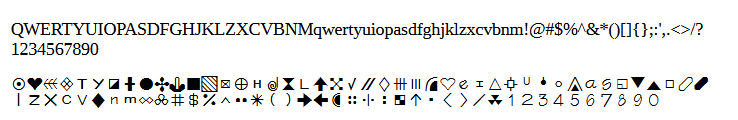
\includegraphics[width=150mm]{font_example.png}
			\caption{Следующим образом будет выглядеть стандартный латинский алфавит и некоторые другие привычные нам символы в этом шрифте}
		}
	\end{figure}
	
	По сути, теперь алгоритм сводится к тому, чтобы пройти по каждой ячейке схемы, полученной выше, считать цвет для каждой ячейки и на основе этого добавить туда один символ текста, соответствующий номеру этого цвета в массиве ключевых цветов.
	
	Здесь стоит подумать о разрешении изображения. При нанесении текста на схему, где размер ячейки составляет, к примеру, 5 пикселей, текст будет, скорее всего, неразличим, а если пользователь увеличит его вручную позднее, сжатость текста будет еще заметнее. Напишем функцию (принимающую уже объект Image из библиотеки Pillow, а не трехмерный массив numpy), которая увеличивает пикселизированное изображение перед нанесением сетки и значков так, чтобы размер ячейки был не меньше 15 пикселей и при этом оставался целым значением. Использующийся в процессе аргумент NEAREST отвечает за тип сглаживания при увеличении размера --- такое сглаживание обеспечивает отсутствие пикселей промежуточных цветов между пикселями исходного изображения, оставляя его максимально близким к оригиналу.
	
	\lstinputlisting[linerange = {149-157}]{progs/picto/with_picto.py}
	
	Еще стоит задуматься о том, какого цвета будут значки. По умолчанию это черный цвет, но для слишком темных цветов он будет сливаться с самой ячейкой. Введем функцию, которая определяет степень яркости ячейки по переданным координатам (эта яркость --- результат сложения компонент цвета, умноженных на зависящие от особенностей человеческого зрения коэффициенты) и возвращает 1, если все-таки целесообразно использовать черный цвет. Такую же функцию можно ввести для всего изображения в целом, чтобы определить подходящий цвет для сетки, а не всегда по умолчанию использовать серый.
	
	Заметим также, что пороги допустимости использования черного для сетки и ячейки существенно разнятся: для сетки мы пытаемся найти некоторую середину, а для ячейки используем черный в большинстве случаев --- опытным путем было выяснено, что слишком частое переключение между черным и светло-серым утомляет глаз.
	
	\lstinputlisting[linerange = {141-147}]{progs/picto/with_picto.py}	
	
	Ну и наконец, так будет выглядеть алгоритм расстановки значков. Мы задаем сам шрифт, помещая файл .ttf в папку, связанную с проектом, и его размер в зависимости от размера ячейки. Также здесь создается строка <<алфавит>> со всеми символами, которые могут использоваться. Поскольку значки наносятся после нанесения сетки, определяем ее размер для вычисления координат ячеек. далее для каждой ячейки перебираем все ключевые цвета, и когда находит точное совпадение, определяем, какой цвет должен использоваться для значка, наносим значок и прерываем цикл перебора цветов.
	
	\lstinputlisting[linerange = {159-173}]{progs/picto/with_picto.py}
	
	В конечном итоге последовательность функций, которую надо выполнить над исходным изображением, будет выглядеть следующим образом.
	
	\lstinputlisting[linerange = {207-236}]{progs/picto/with_picto.py}
	
	Здесь, помимо прочего, вносится важное изменение: теперь с клавиатуры вводится не размер ячейки в пикселях, а  ширина и высота схемы в ячейках. Один из параметров можно оставить пустым: тогда второй будет автоматически вычислен как пропорциональный ему. Если же ввести два параметра, изображение будет обрезано, чтобы соответствовать указанным пропорциям. Это достигается следующими функциями.
	
	\lstinputlisting[linerange = {34-50}]{progs/picto/with_picto.py}
	
	\hyperref[with_picto_cats]{Результаты} этого этапа также представлены в приложении. 
	
	\subsection{Соответствие между цветами и нитками}
	
	Усовершенствуем нашу программу так, чтобы она окрашивала схему не прост ов цвета, которые встречаются в ней чаще всего, а в цвета, соответствующие ниткам, которые максимально близко --- но не всегда точно --- повторяют этот цвет. Само собой, для этого понадобится каким-то образом переводить цвета в коды ниток в некоторой палитре. Самостоятельно составлять таблицы соответствий ниток и цветов в системе RGB весьма утомительная работа. К счастью, на сайтах, посвященных рукоделию, можно найти уже готовые таблицы. Скопируем в текстовый файл такую таблицу для палитры ниток DMC (ознакомиться с ним можно в разделе приложений).
	
	Как считывать информацию оттуда? Строки, соответствующие отдельным цветам, разбиты символом <<\\n>>, а параметры каждого цвета --- символом <<\\t>>. В принципе, используя стандартные функции для работы с файлами, можно считывать эти данные, разбивать на отдельные значения с помощью метода split и работать с ними. Но есть более удобный способ представления таких данных --- формат JSON. JSON, что расшифровывается как JavaScript Object Notation — это открытый, независимый от языка программирования, стандартный формат файла для обмена данными. В нем для хранения и передачи данных используется удобочитаемый текст, поскольку внутрення структура использует уже знакомые модели массива и объекта. Файлы JSON хранятся с расширением .json. 

	Таким образом, мы можем написать вспомогательную программу, с ее помощью единожды обработать текстовый файл, создать на его основе файл .json и в дальнейшем использовать в программе именно его. В таком подходе есть очевидные преимущества: сведения об одном цвете можно хранить не в массиве, а в словаре, обращаясь к его свойствам по строковым обозначениям --- что делает процесс чтения легче для восприятия.
	
	\lstinputlisting{DMC/createJSON.py}
	
	Далее поступим следующим образом: определим две функции, первая из которых будет на основе массива ключевых цветов создавать массив словарей, содержащих информацию о цветах из палитры ниток, наиболее близких к ключевым цветам. Если в массиве ключевых цветов есть очень близкие оттенки, и два цвета соответствуют одному и тому же цвету нитки, то цвет включается только единожды. Соответственно, когда мы работаем с палитрой ниток, мы можем получить изображение с меньшим, чем заданное, количеством цветов. И это разумно: в палитре может в принципе не содержаться заданное количество цветов, чтобы представить именно это изображение. Вторая функция будет из массива всей информации об используемых нитках извлекать только массивы, отображающие цвета: такой массив можно будет без проблем передавать функциям перекраски изображения и нанесения значков, и при передаче схема будет изменяться в соответствии с массивом ниток.
	
	\lstinputlisting[linerange = {128-150}]{progs/relating_with_threads/relating_with_threads.py}
	
	Помимо этого, хотелось бы выводить на схему информацию об используемых нитках: как соотносятся используемые цвета и значки с кодовым номером и наименованием используемых ниток. В конце концов, если в наличии у пользователя таких цветов нет, а он захочет приобрести их, он должен знать, как найти их в каталоге. Для этого нам нужно будет создать новое изображение, с полями внизу, а также по бокам, но только в том случае, если само изображение слишком мало, чтобы в строку под ним вмещались сведения хотя бы о двух цветах. Затем на эти поля наносится информация --- ячейка заданного цвета и с заданным значком, номер и название тона.	В данную функцию будет передаваться массив со всеми данными об используемых нитках.
	
	\lstinputlisting[linerange = {220-249}]{progs/relating_with_threads/relating_with_threads.py}
	
	Однако, как мы уже говорили, использование функций для перевода массива ключевых цветов в массив ниток приводит к искажению палитры --- количество цветов может сократиться, а цвета ниток не идеально совпадают с выделенными алгоритмом k-means цветами. Тем временем, в мире существуют и другие палитры ниток, а также пользователь может попробовать получить нужный цвет сам, например, их смешением. В таком случае, он может захотеть получить схему, где используются просто ключевые цвета. Так можно поступить, если написанным в предыдущих разделах функциям по-прежнему передавать не измененный массив ключевых цветов. Что до вывода доп. информации в таком случае, будет полезно просто вывести используемые цвета отдельно от значков, давая пользователю возможность увидеть их чистыми и подобрать наиболее близкий оттенок самостоятельно. Для этого напишем облегченную версию функции выше: она уже не рассматривает сценарий <<добавить поля по бокам>>, потому что такая информация априори не может занимать много места, и имеющейся ширины всегда будет хватать.
	
	\lstinputlisting[linerange = {251-274}]{progs/relating\_with\_threads/relating_with_threads.py}	
	
	В конечном итоге последовательность функций, которую надо выполнить над исходным изображением, будет выглядеть следующим образом. Нам потребуется вводить с клавиатуры дополнительный параметр, отвечающий за то, строится ли схема с заменой цветов на нитки. В зависимости от этого меняются вызываемые функции и передаваемые им версии массива цветов.
	
	\lstinputlisting[linerange = {277-324}]{progs/relating\_with\_threads/relating\_with\_threads.py}	
	
	\hyperref[with_info_cats]{Эти результаты} также доступны в приложении.
	
	\subsection{Заключительная версия программы:}
	
	Наконец, можем представить заключительную версию программы. В ней все вспомогательные файлы объединены в один с ней каталог, введены проверки некоторых сценариев, которые могут вызвать ошибку в работе программы, ввод сопровожден комментариями, и в целом удалены некоторые ограничения и условности, накладываемые версией для тестирования.
	
	\lstinputlisting{progs/final/final_making_scheme.py}	
	
	\section{Вывод:}
	
	Можно ли сказать, что поставленные цели выполнены? В целом да: мы получили не одну схему, удовлетворяющую условиям, поставленным вначале, и рассмотрели процесс формирования на всех этапах. Есть ли направления, где возможно улучшение написанного кода? Безусловно. К примеру, можно снабдить эту программу более удобным графическим интерфейсом вместо взаимодействия через консоль; можно более тщательно заняться вопросами оптимизации, можно добавить новые элементы функционала --- например, добавление в список ключевых цветов некоторых заранее зарезервированных, что в принципе позволяет алгоритм k-means. Так что потенциал для дальнейшего развития у темы есть, и возможно, мы еще вернемся к ней в будущем.
	
	
	\section{Список используемых источников:}
	
	\begin{thebibliography}{99}
		\bibitem{latexbible} Воронцов~К.В. \LaTeX 2$_\varepsilon$ в примерах.
		--- 16 декабря 2005.
		\bibitem{basecourse} Pillow: обработка изображений в Python на примерах; python-scripts.com
		\bibitem{maincourse} Image Module documentation; pillow.readthedocs.io
		\bibitem{maincourse2} ImageDraw Module documentation; pillow.readthedocs.io
		\bibitem{habr1} Наглядно о том, как работает NumPy; habr.com
		\bibitem{habr2} Кластеризация палитры изображения и сжатие в формате PNG; habr.com
		\bibitem{useless} Краткий курс теории обработки изображений; hub.exponenta.ru
	\end{thebibliography}
	
	\section{Приложения (Фотографии):}
	\label{assets}
	
	\begin{figure}[bh]
		\noindent\centering{
			
\includegraphics[width=130mm]{images/origins/cats.png}
			\caption{Изображение по умолчанию cats.png}
		}
	\end{figure}
	\label{cats}

	\begin{figure}[bh]
		\noindent\centering{
			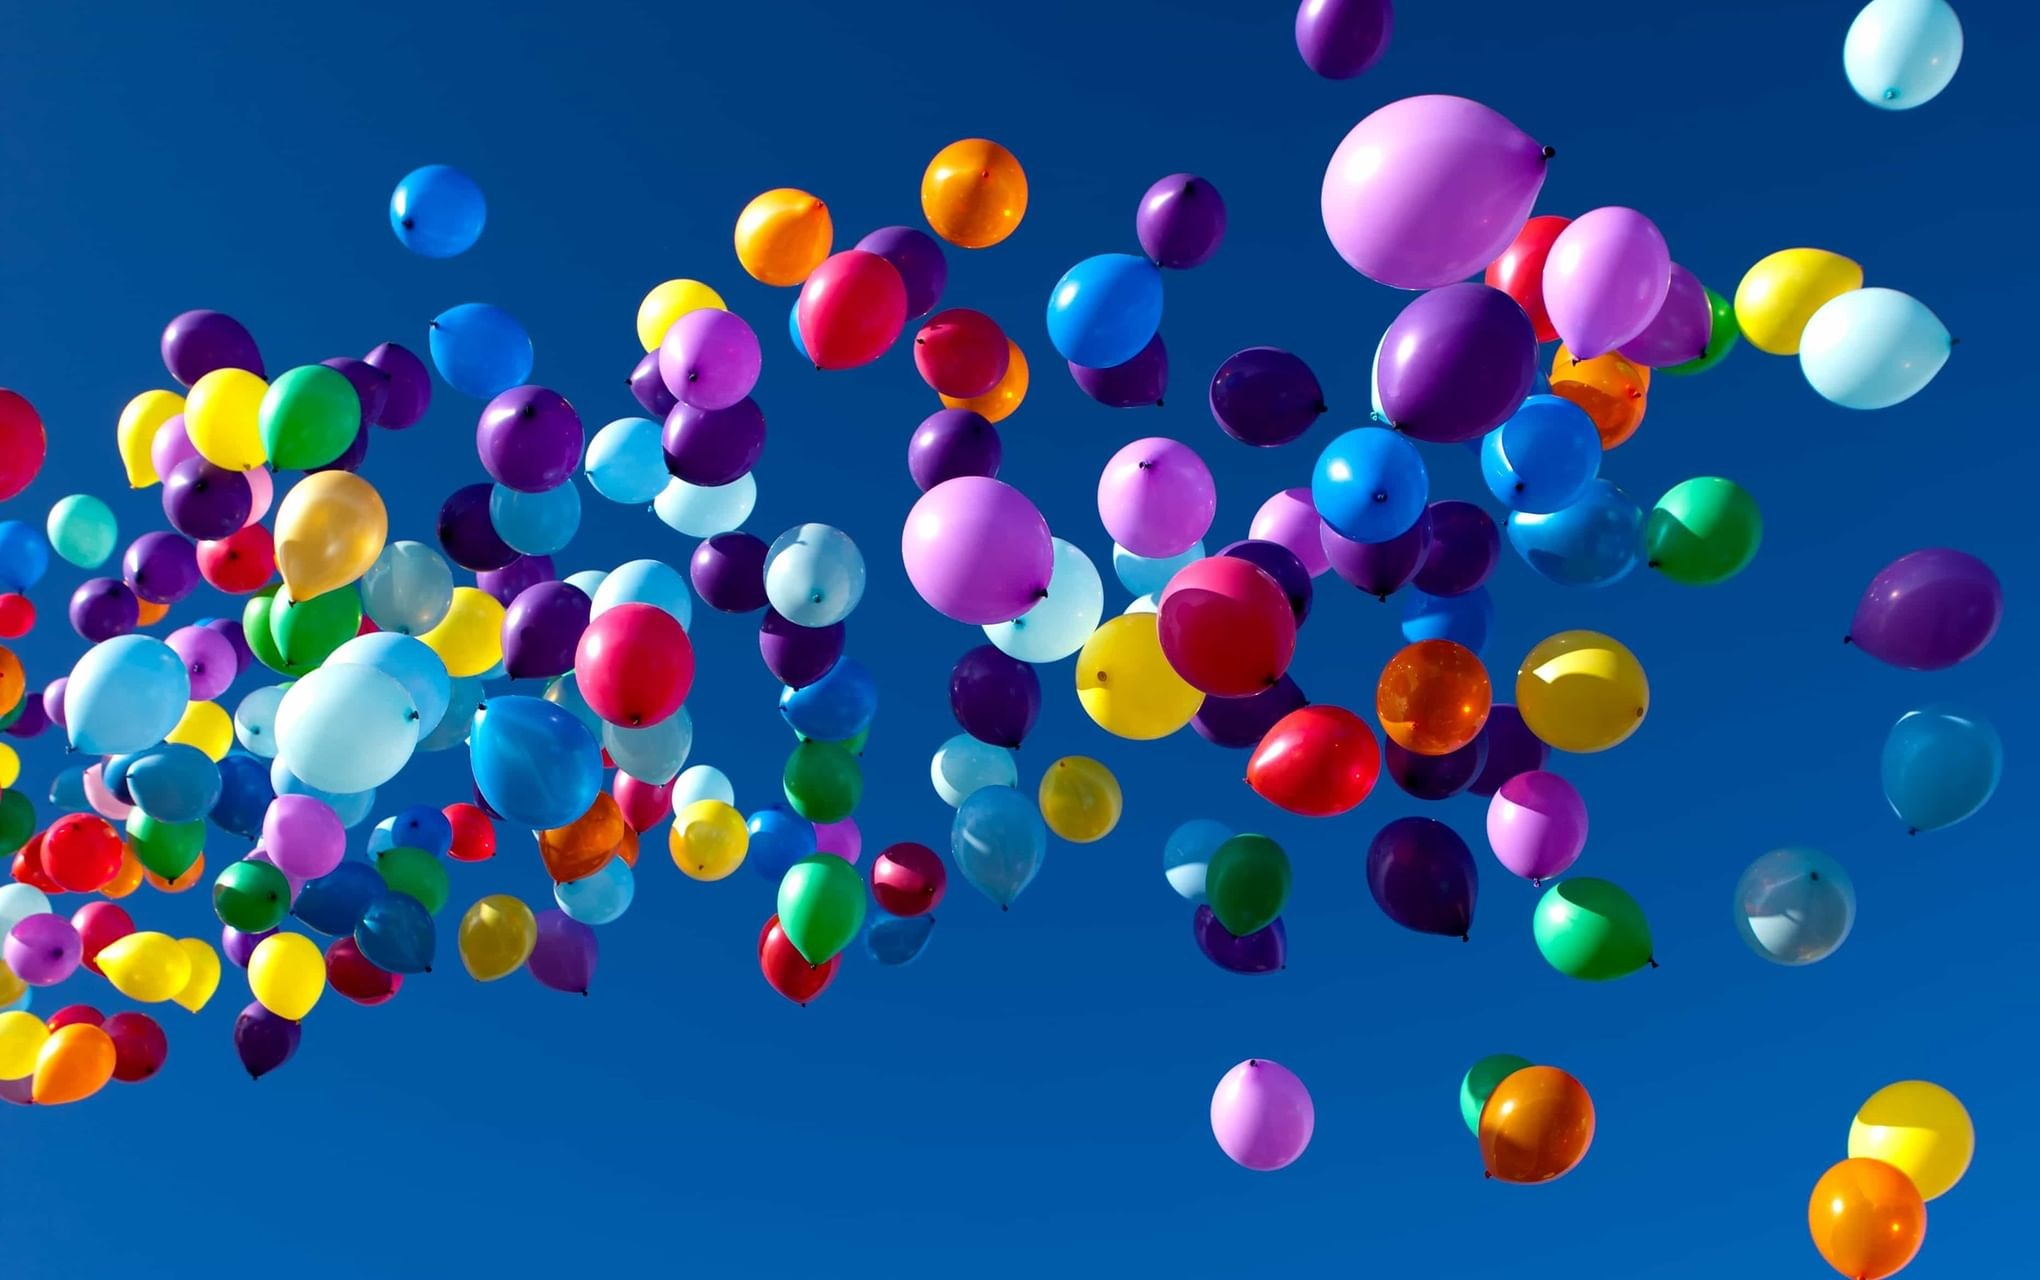
\includegraphics[width=150mm]{images/origins/baloons.png}
			\caption{Изображение по умолчанию baloons.png}
		}
	\end{figure}
	\label{baloons}	
	
	\begin{figure}[bh]
		\noindent\centering{
			
\includegraphics[width=100mm]{images/origins/imp.png}
			\caption{Изображение по умолчанию imp.png}
		}
	\end{figure}
	\label{imp}		
	
	\begin{figure}[bh]
		\noindent\centering{
			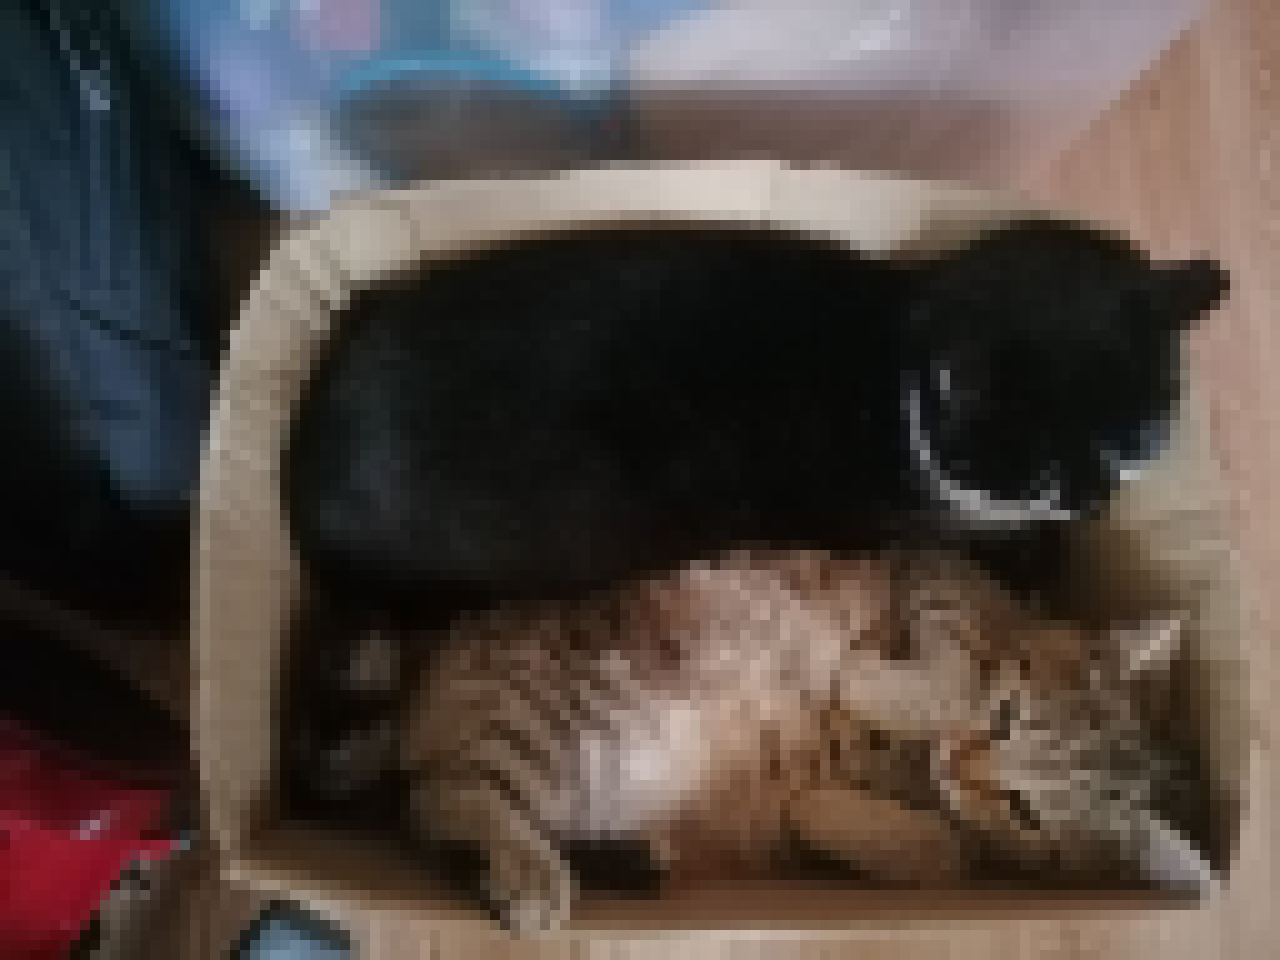
\includegraphics[width=130mm]{images/generals/pixel_cats.png}
			\caption{Пикзелизированное изображение cats.png с размером ячейки 10}
		}
	\end{figure}
	\label{pixel_cats}
	
	\begin{figure}[bh]
		\noindent\centering{
			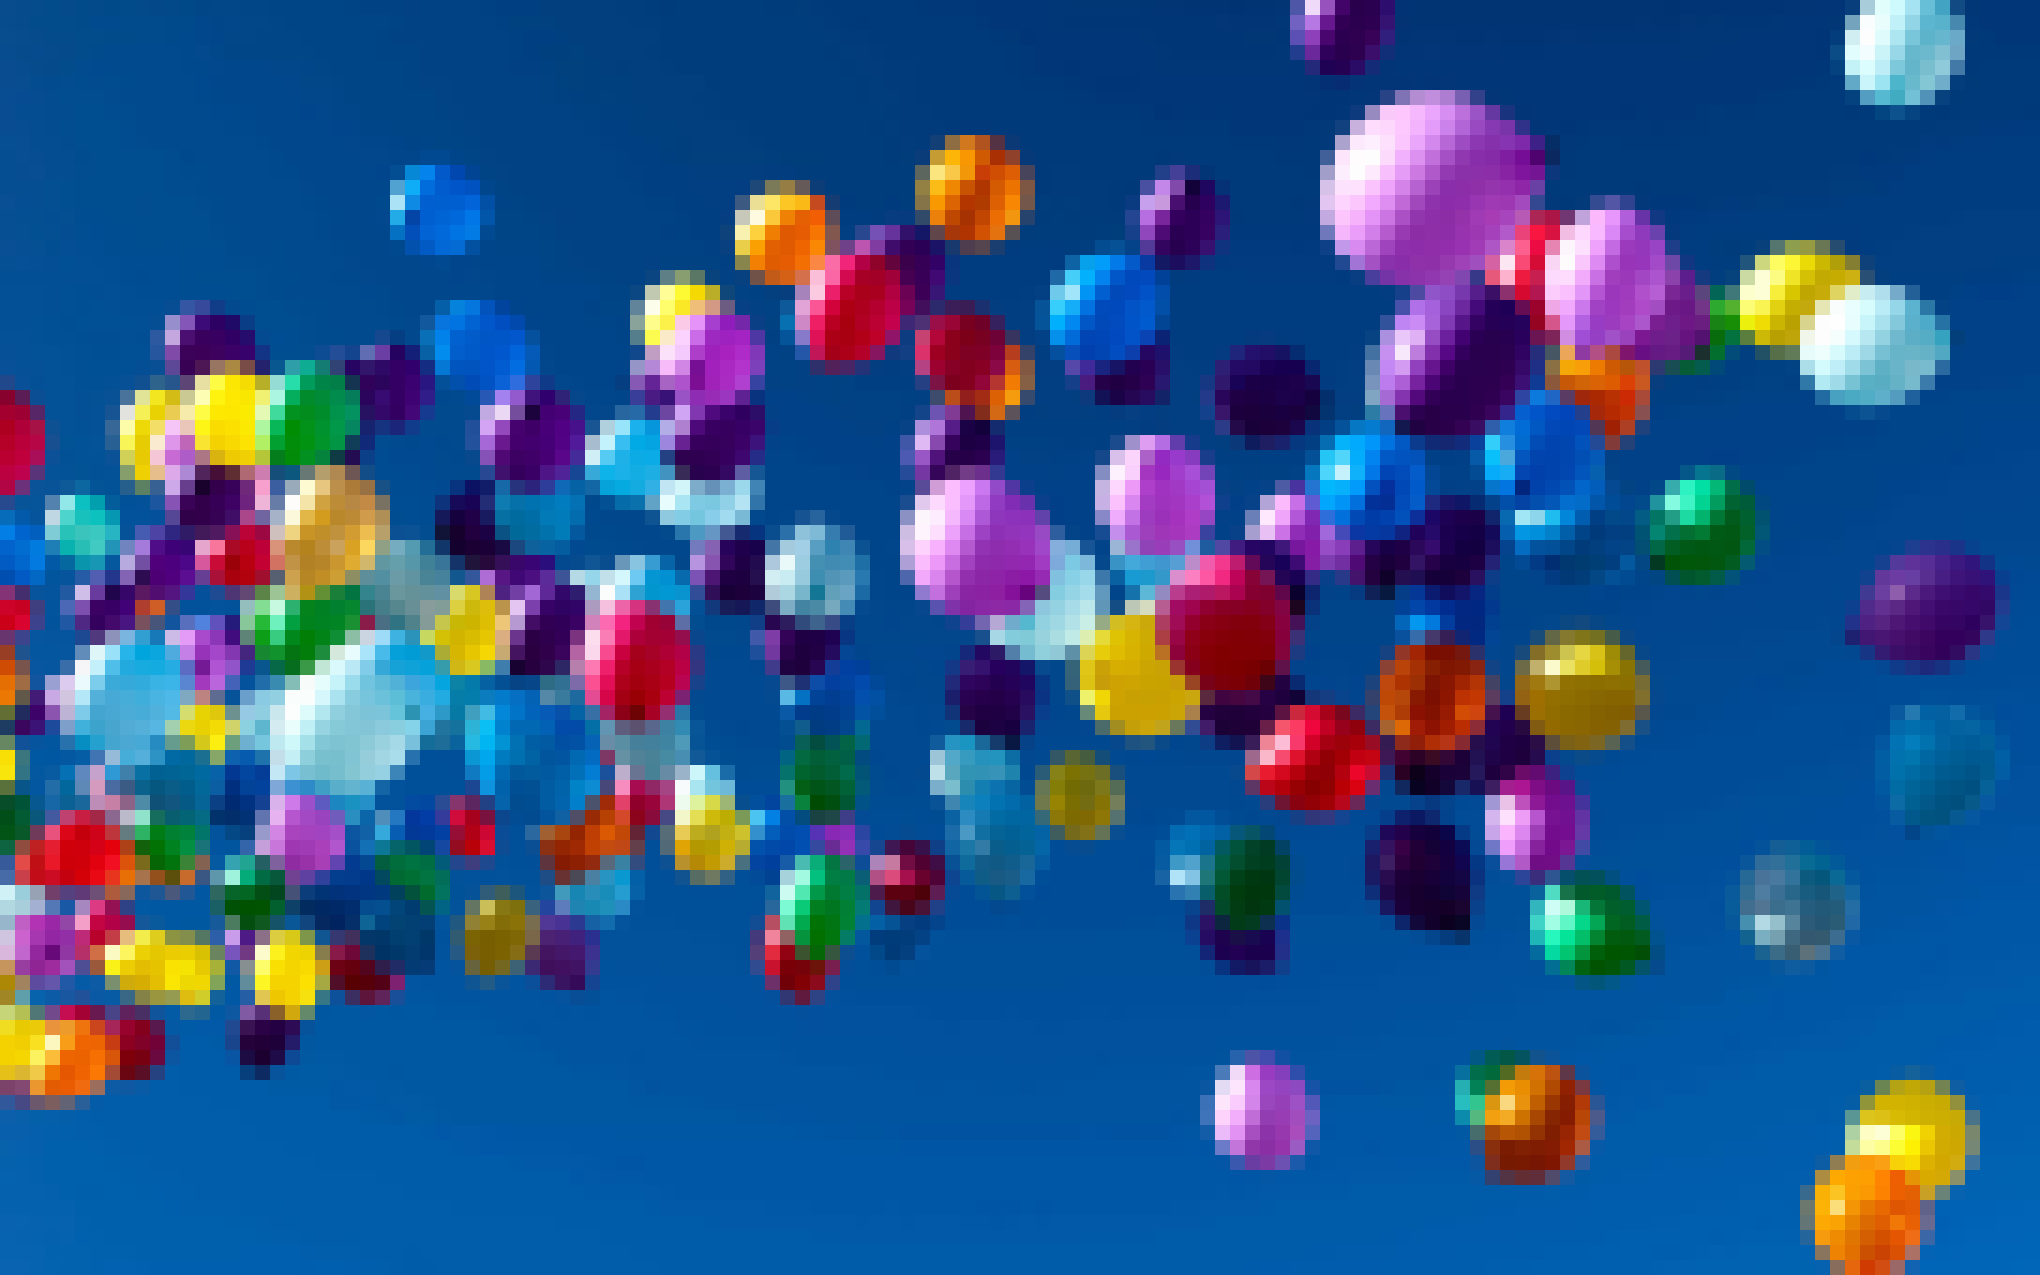
\includegraphics[width=150mm]{images/generals/pixel_baloons.png}
			\caption{Пикзелизированное изображение baloons.png с размером ячейки 15 (размеры изображения не кратны ему)}
		}
	\end{figure}
	\label{pixel_baloons}	
	
	\begin{figure}[bh]
		\noindent\centering{
			
\includegraphics[width=100mm]{images/generals/pixel_imp.png}
			\caption{Пикзелизированное изображение imp.png с размером ячейки 6 (размеры изображения не кратны ему)}
		}
	\end{figure}
	\label{pixel_imp}	
	
	\begin{figure}[bh]
		\noindent\centering{
			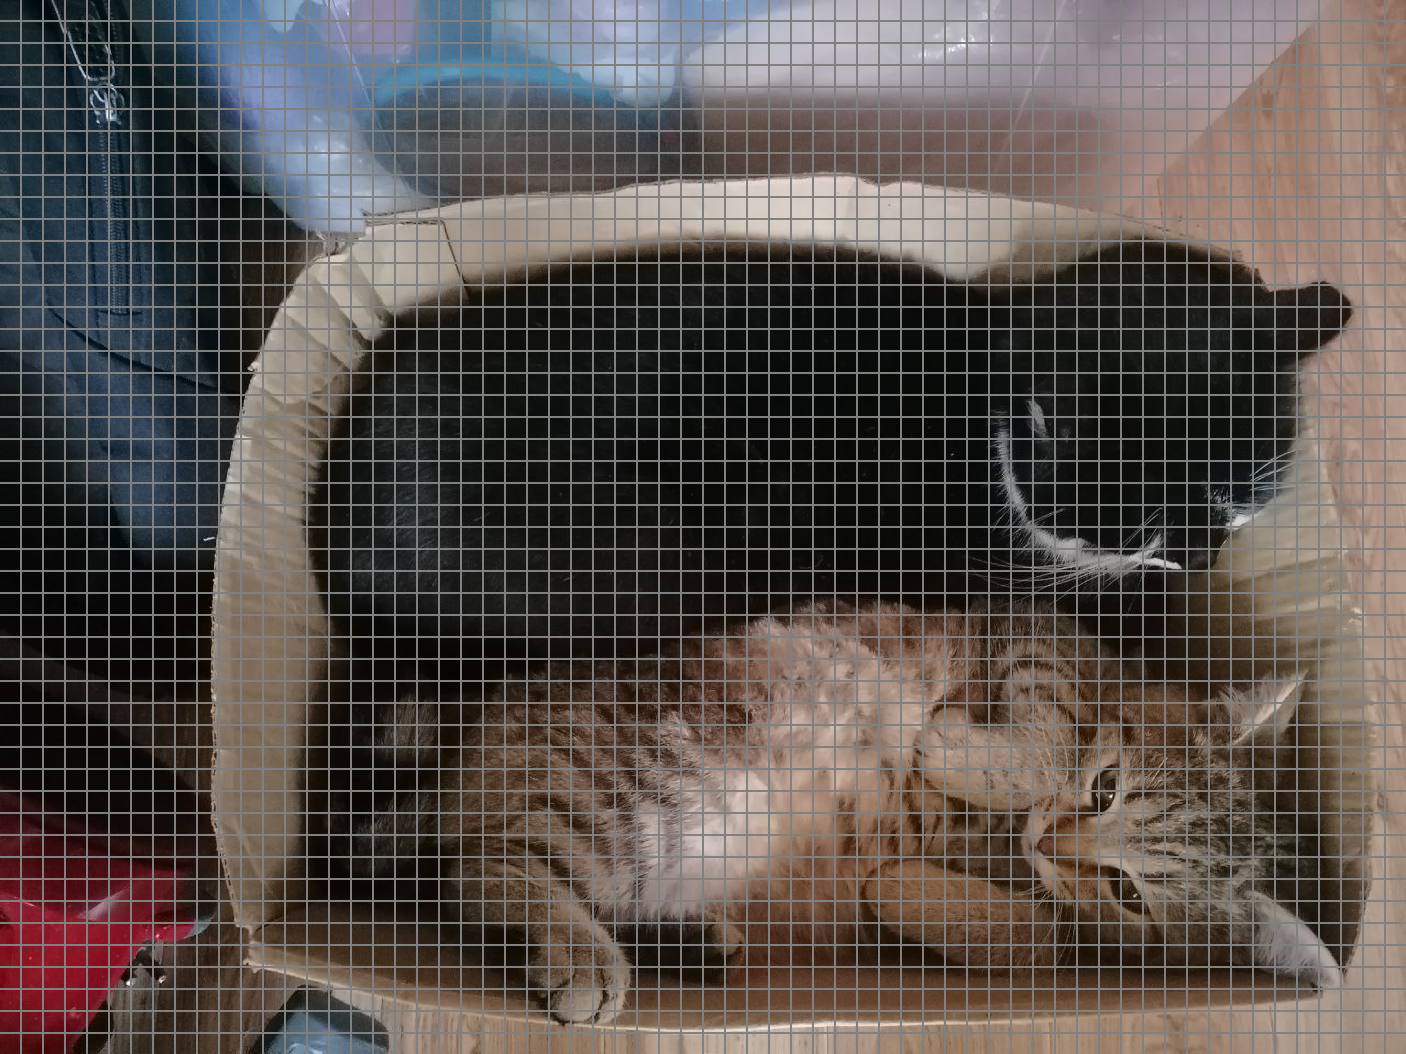
\includegraphics[width=130mm]{images/generals/gridded_cats.png}
			\caption{Покрытое сеткой изображение cats.png с размером ячейки 20 (размер прутьев сетки = 20/2 = 2)}
		}
	\end{figure}
	\label{gridded_cats}
	
	
	\begin{figure}[bh]
		\noindent\centering{
			
\includegraphics[width=100mm]{images/generals/gridded_imp.png}
			\caption{Покрытое сеткой изображение imp.png с размером ячейки 6 (размер прутьев сетки 1)}
		}
	\end{figure}
	\label{gridded_imp}	
	
	
	\begin{figure}[bh]
		\noindent\centering{
			
\includegraphics[width=130mm]{images/reduced/reduced_cats.png}
			\caption{Изображение cats.png с сокращенной до 20 цветов палитрой}
		}
	\end{figure}
	\label{reduced_cats}
	
	\begin{figure}[bh]
		\noindent\centering{
			
\includegraphics[width=150mm]{images/reduced/reduced_baloons.png}
			\caption{Изображение baloons.png с сокращенной до 20 цветов палитрой}
		}
	\end{figure}
	\label{reduced_baloons}	
	
	\begin{figure}[bh]
		\noindent\centering{
			
\includegraphics[width=100mm]{images/reduced/reduced_imp.png}
			\caption{Изображение imp.png с сокращенной до 20 цветов палитрой}
		}
	\end{figure}
	\label{reduced_imp}
	}
	
	\begin{figure}[bh]
		\noindent\centering{
			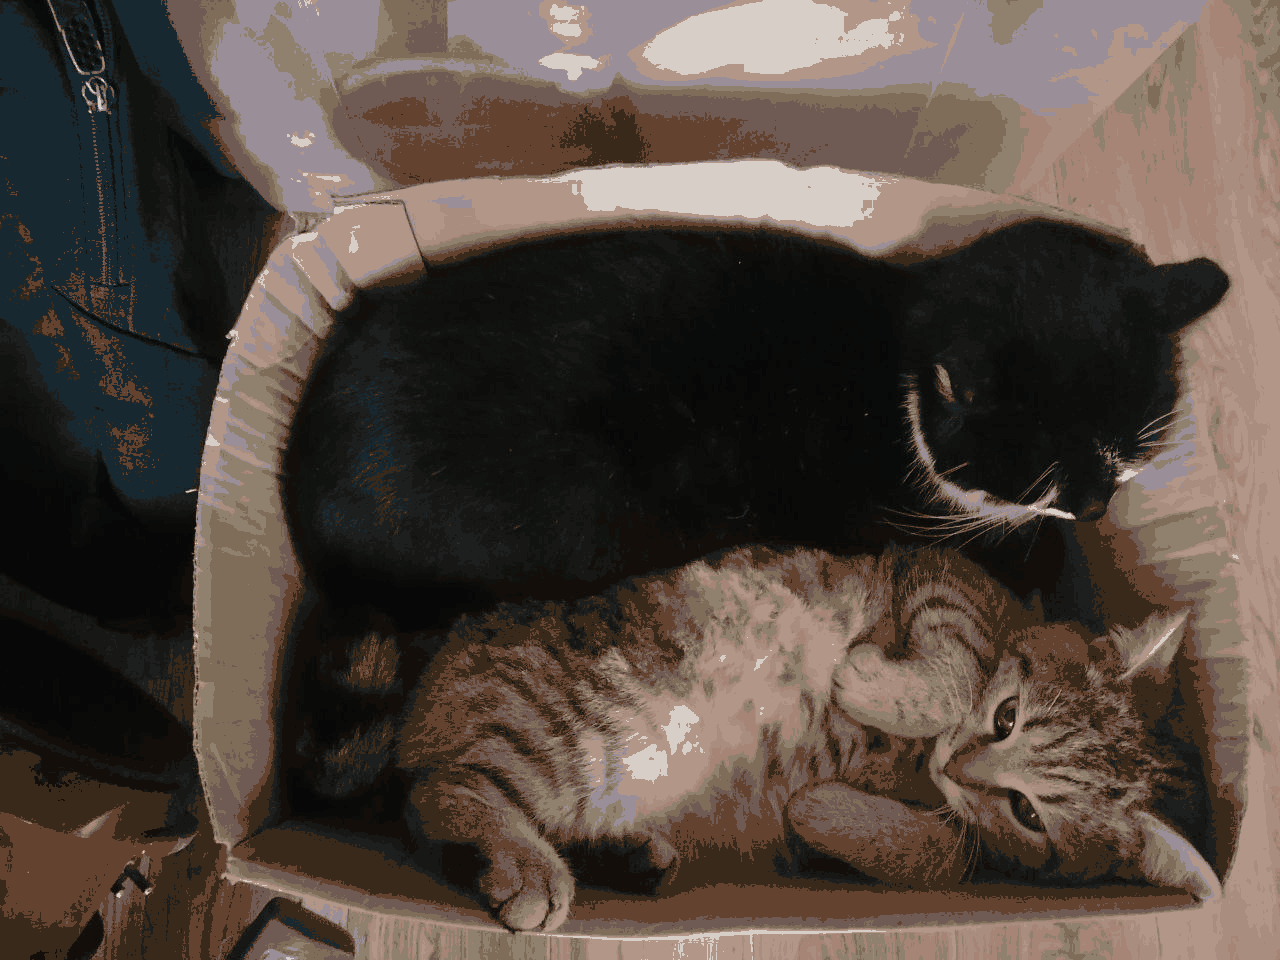
\includegraphics[width=130mm]{images/reduced/reduced_with_step_20_1.0_cats.png}
			\caption{Изображение cats.png с сокращенной до 20 цветов палитрой (коэффициент зоны 1)}
		}
	\end{figure}
	\label{reduced_with_step_cats}
	
	\begin{figure}[bh]
		\noindent\centering{
			
\includegraphics[width=100mm]{images/reduced/reduced_with_step_20_1.5_imp.png}
			\caption{Изображение imp.png с сокращенной до 20 цветов палитрой (коэффициент зоны 1.5)}
		}
	\end{figure}
	\label{reduced_with_step_imp}
	
	
	\begin{figure}[bh]
		\noindent\centering{
			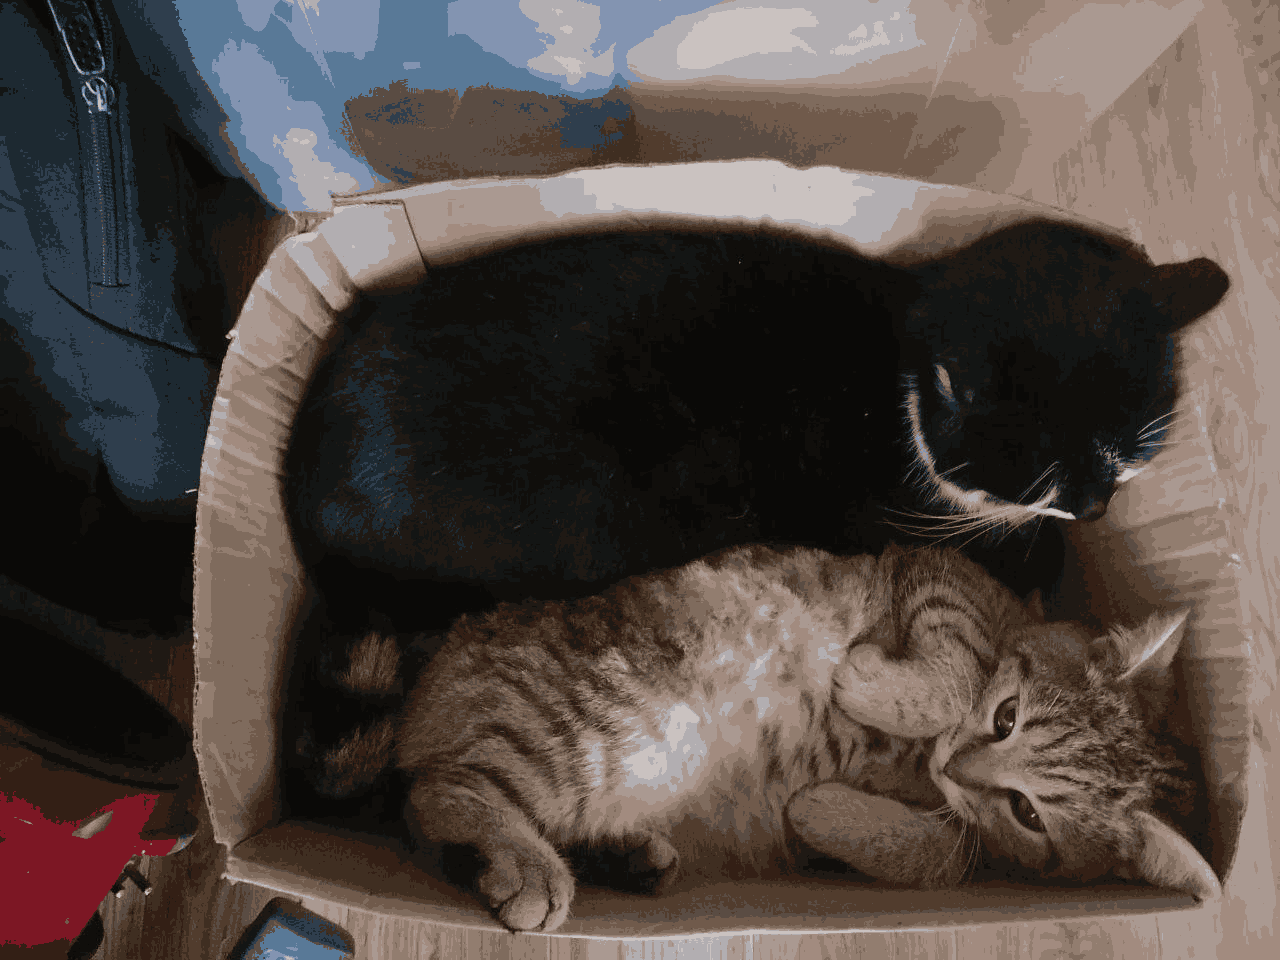
\includegraphics[width=130mm]{images/reduced_clasters/K-means_reduced_20_cats.png}
			\caption{Изображение cats.png с сокращенной методом k-средних до 20 цветов палитрой}
		}
	\end{figure}
	\label{reduced_clasters_cats}
	
	\begin{figure}[bh]
		\noindent\centering{
			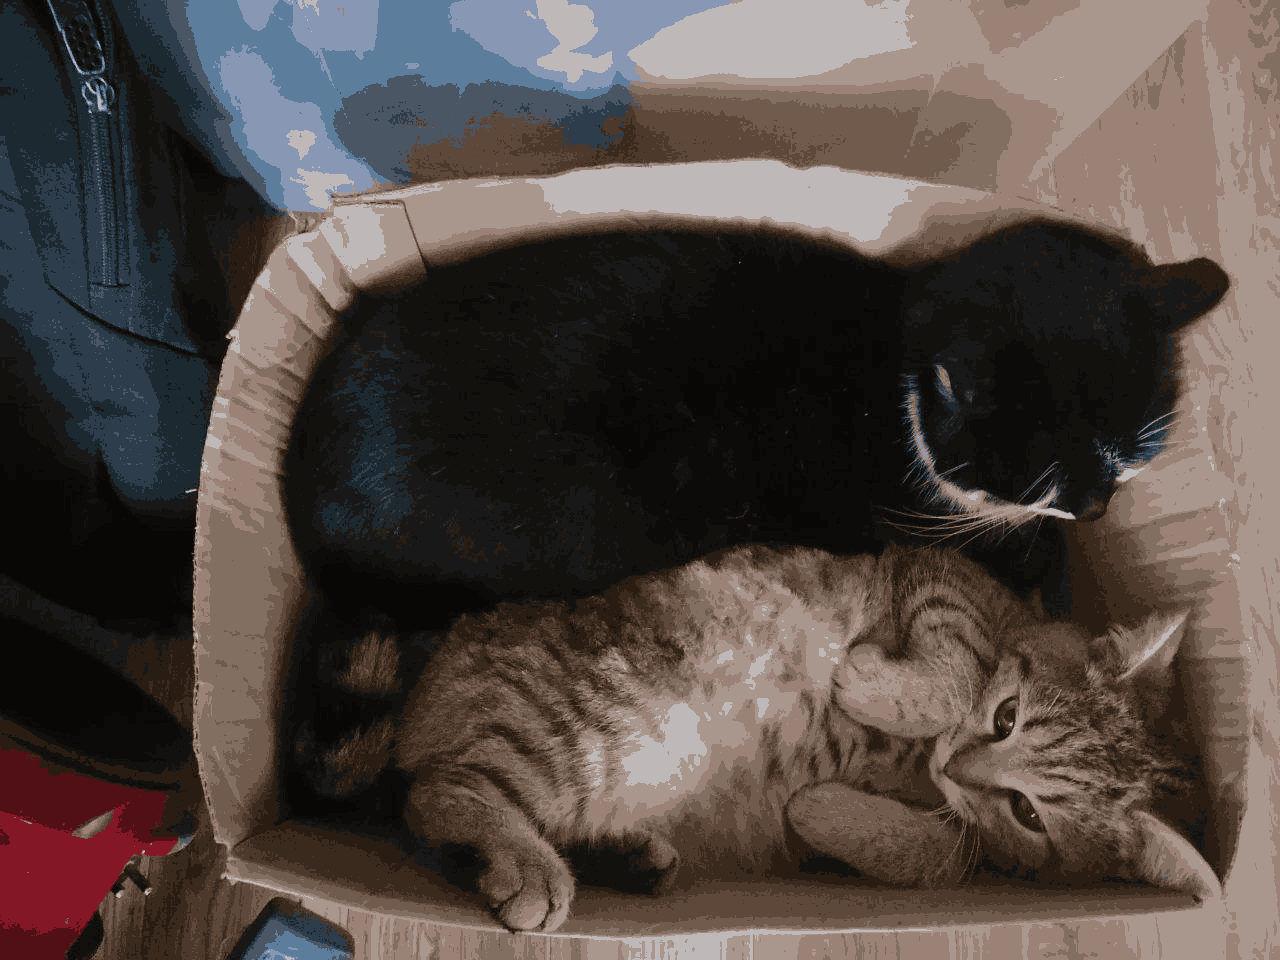
\includegraphics[width=130mm]{images/reduced_clasters/HEXcode_K-means_reduced_20_cats.png}
			\caption{Изображение cats.png с сокращенной методом k-средних до 20 цветов палитрой (использование словаря)}
		}
	\end{figure}
	\label{reduced_clasters_hex_cats}
	
	\begin{figure}[bh]
	\noindent\centering{
		
\includegraphics[width=100mm]{images/reduced_clasters/HEXcode_K-means_reduced_20_imp.png}
			\caption{Изображение imp.png с сокращенной методом k-средних до 20 цветов палитрой (использование словаря)}
	}
	\end{figure}
	\label{reduced_clasters_hex_imp}
	
	\begin{figure}[bh]
		\noindent\centering{
			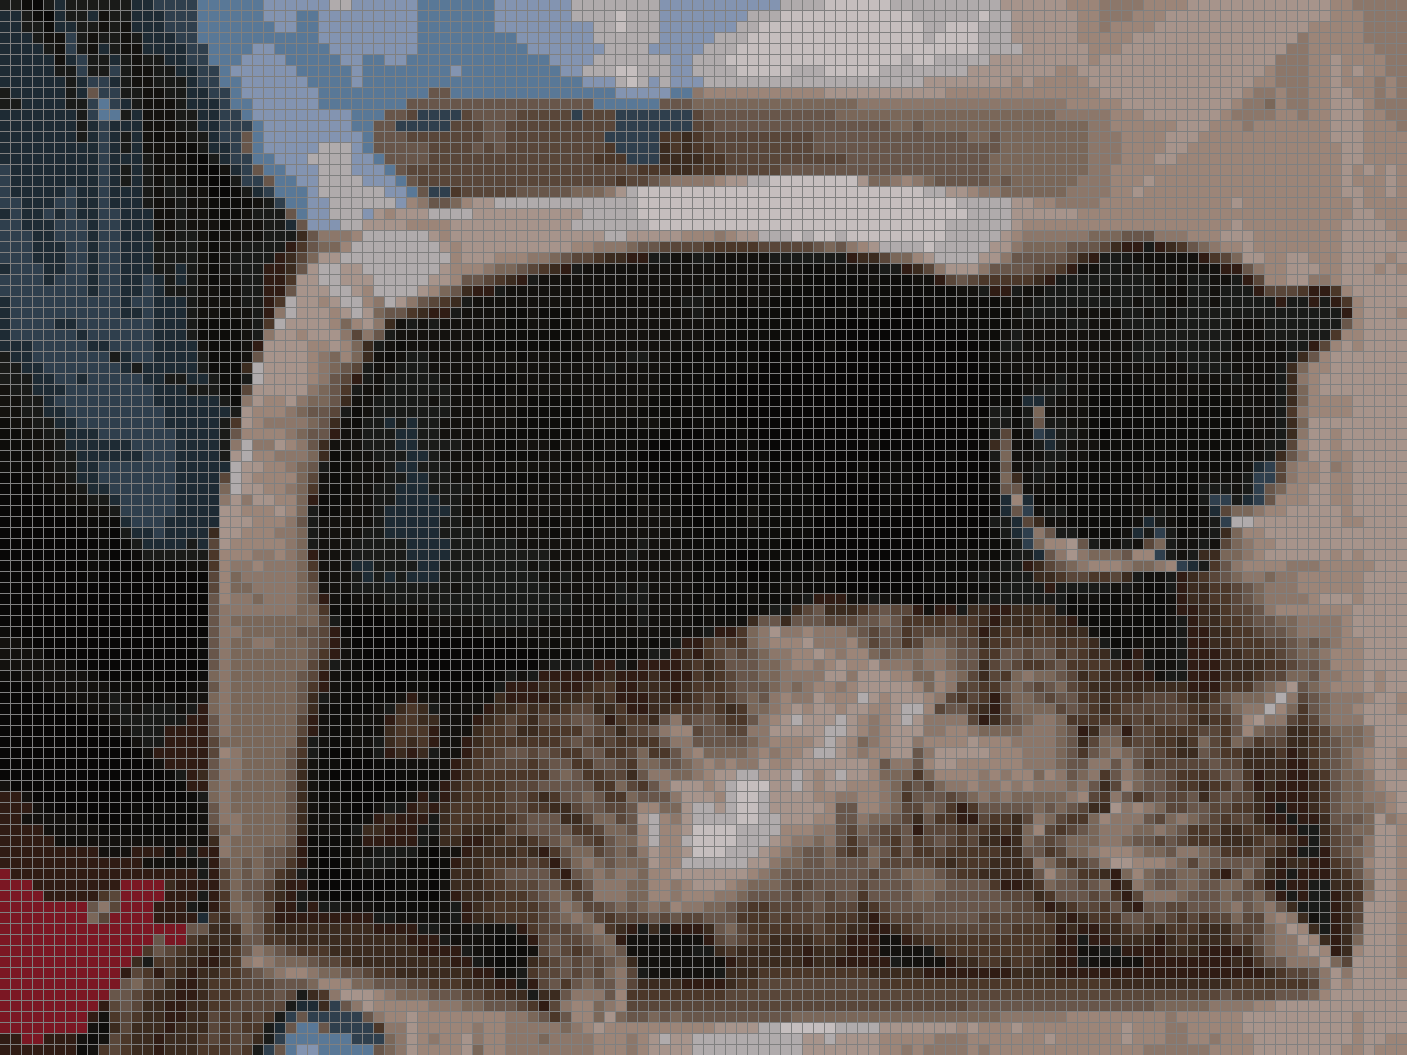
\includegraphics[width=130mm]{images/refactoring1/refactored_cats.png}
			\caption{Первый вариант схемы из 20 цветов и размером ячейки 10 для изображения cats.png}
		}
	\end{figure}
	\label{refactoring1_cats}
	
	\begin{figure}[bh]
		\noindent\centering{
			
\includegraphics[width=100mm]{images/refactoring1/refactored_imp.png}
			\caption{Первый вариант схемы из 20 цветов и размером ячейки 10 для изображения imp.png}
		}
	\end{figure}
	\label{refactoring1_imp}
	
	\begin{figure}[bh]
		\noindent\centering{
			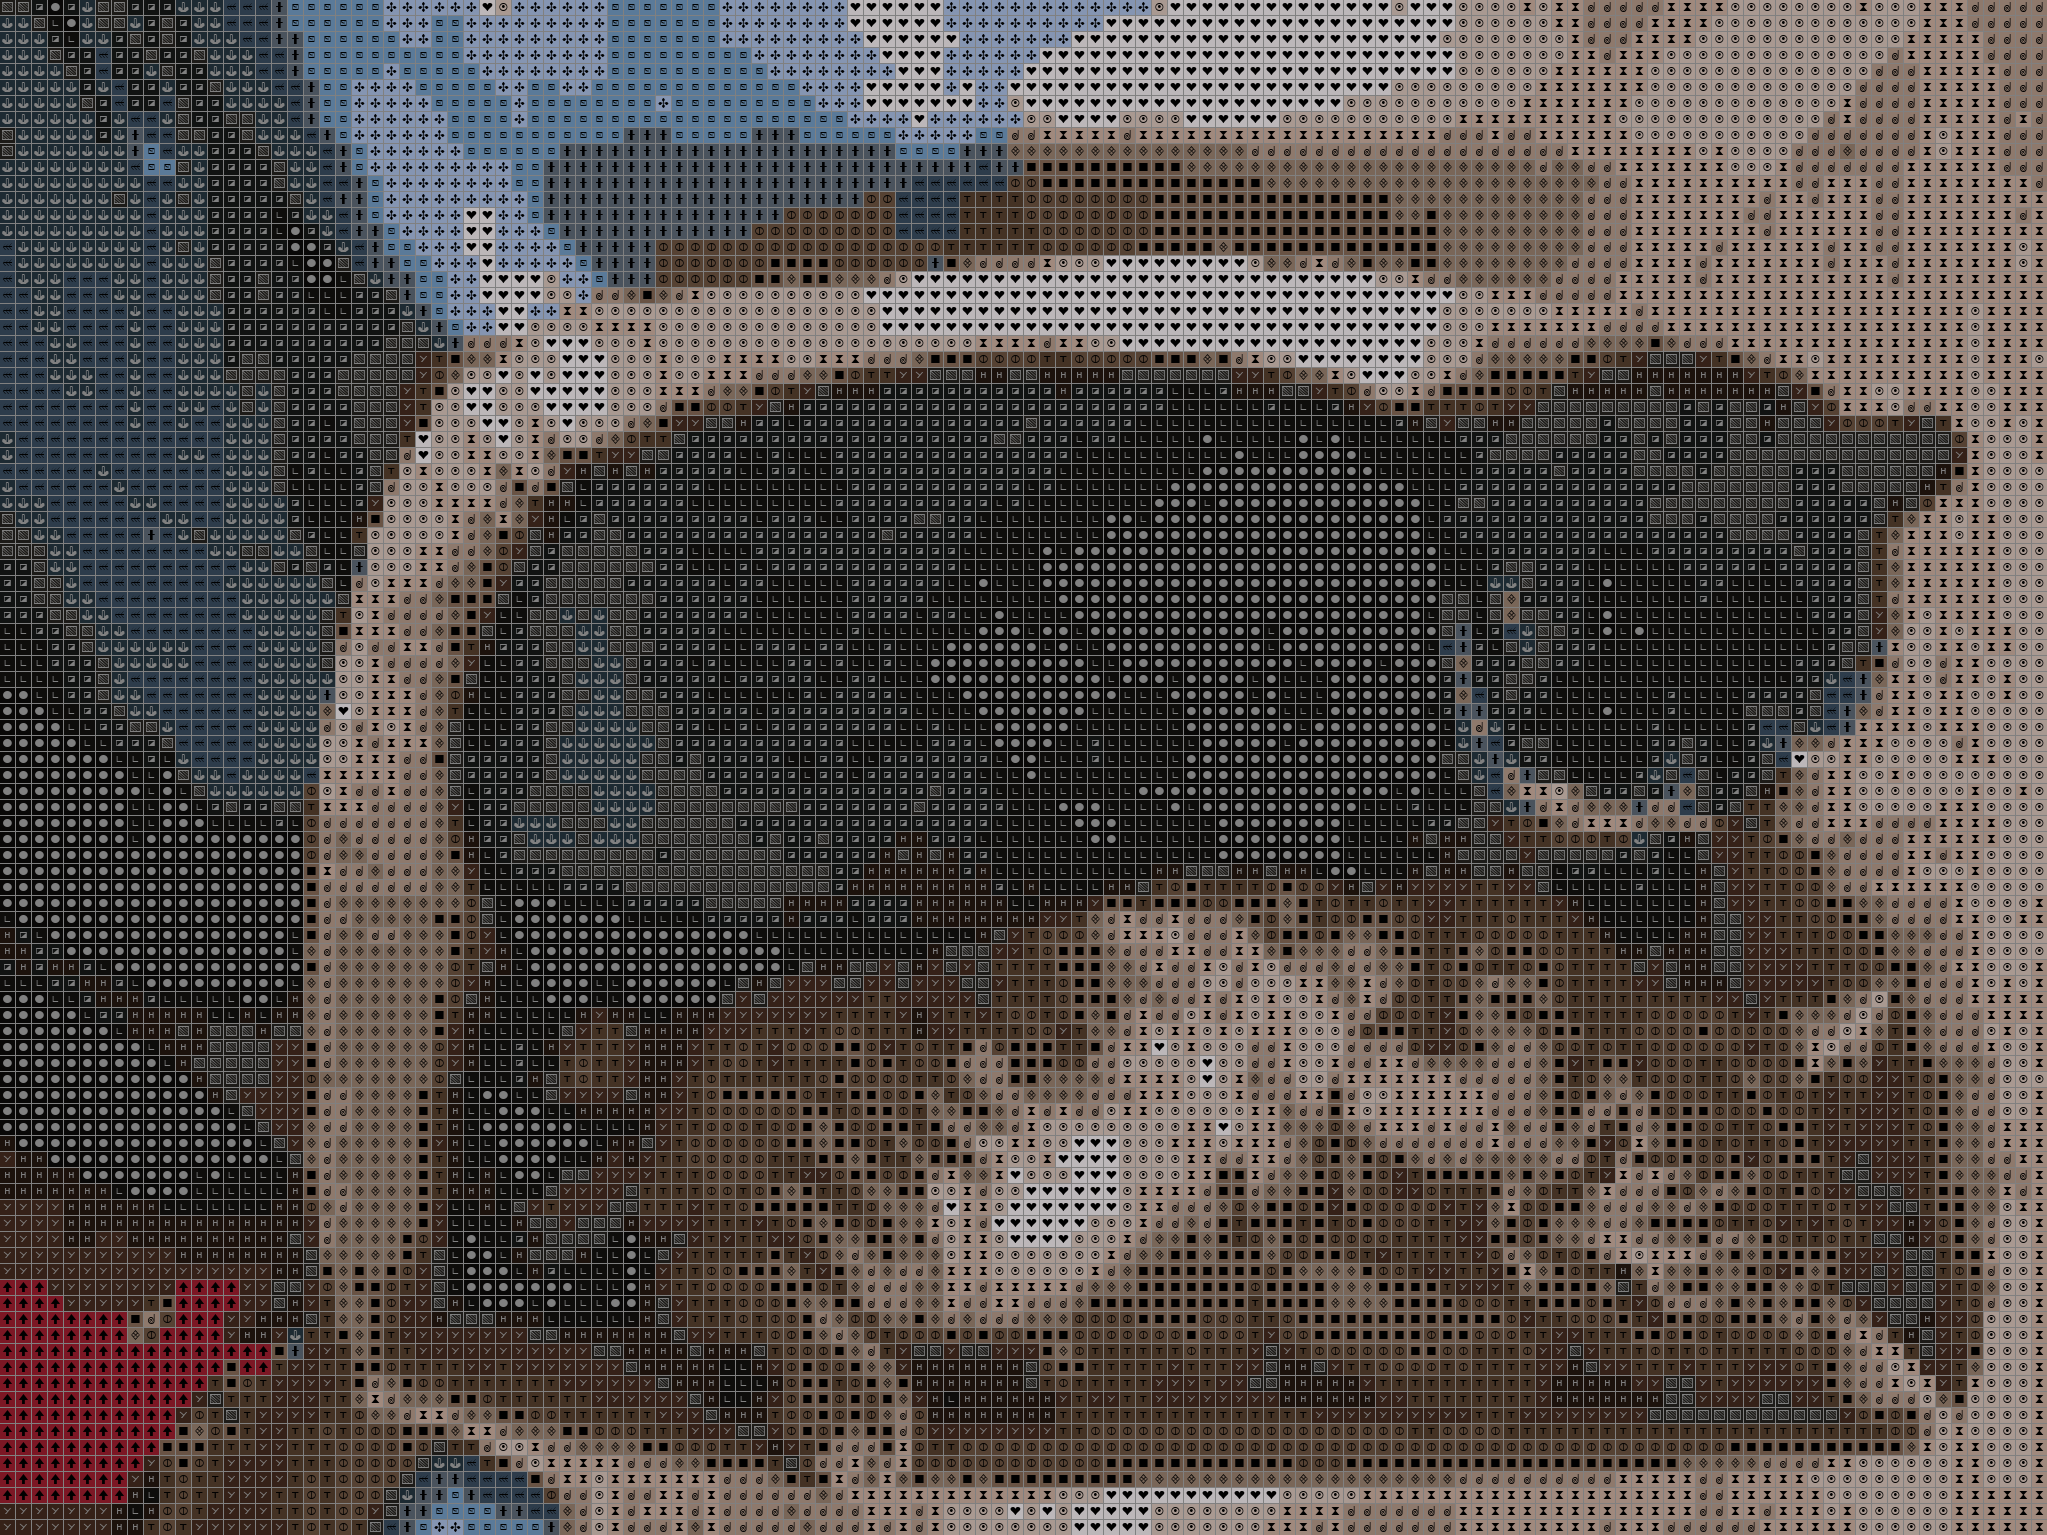
\includegraphics[width=130mm]{images/refactoring1/with_picto_cats.png}
			\caption{Вариант той же схемы, что и выше, но со значками для изображения cats.png}
		}
	\end{figure}
	\label{with_picto_cats}
	
	\begin{figure}[bh]
		\noindent\centering{
			
\includegraphics[width=130mm]{images/refactoring1/with_picto_imp.png}
			\caption{Вариант схемы со значками для изображения imp.png}
		}
	\end{figure}
	\label{with_picto_imp}
	
	\begin{figure}[bh]
		\noindent\centering{
			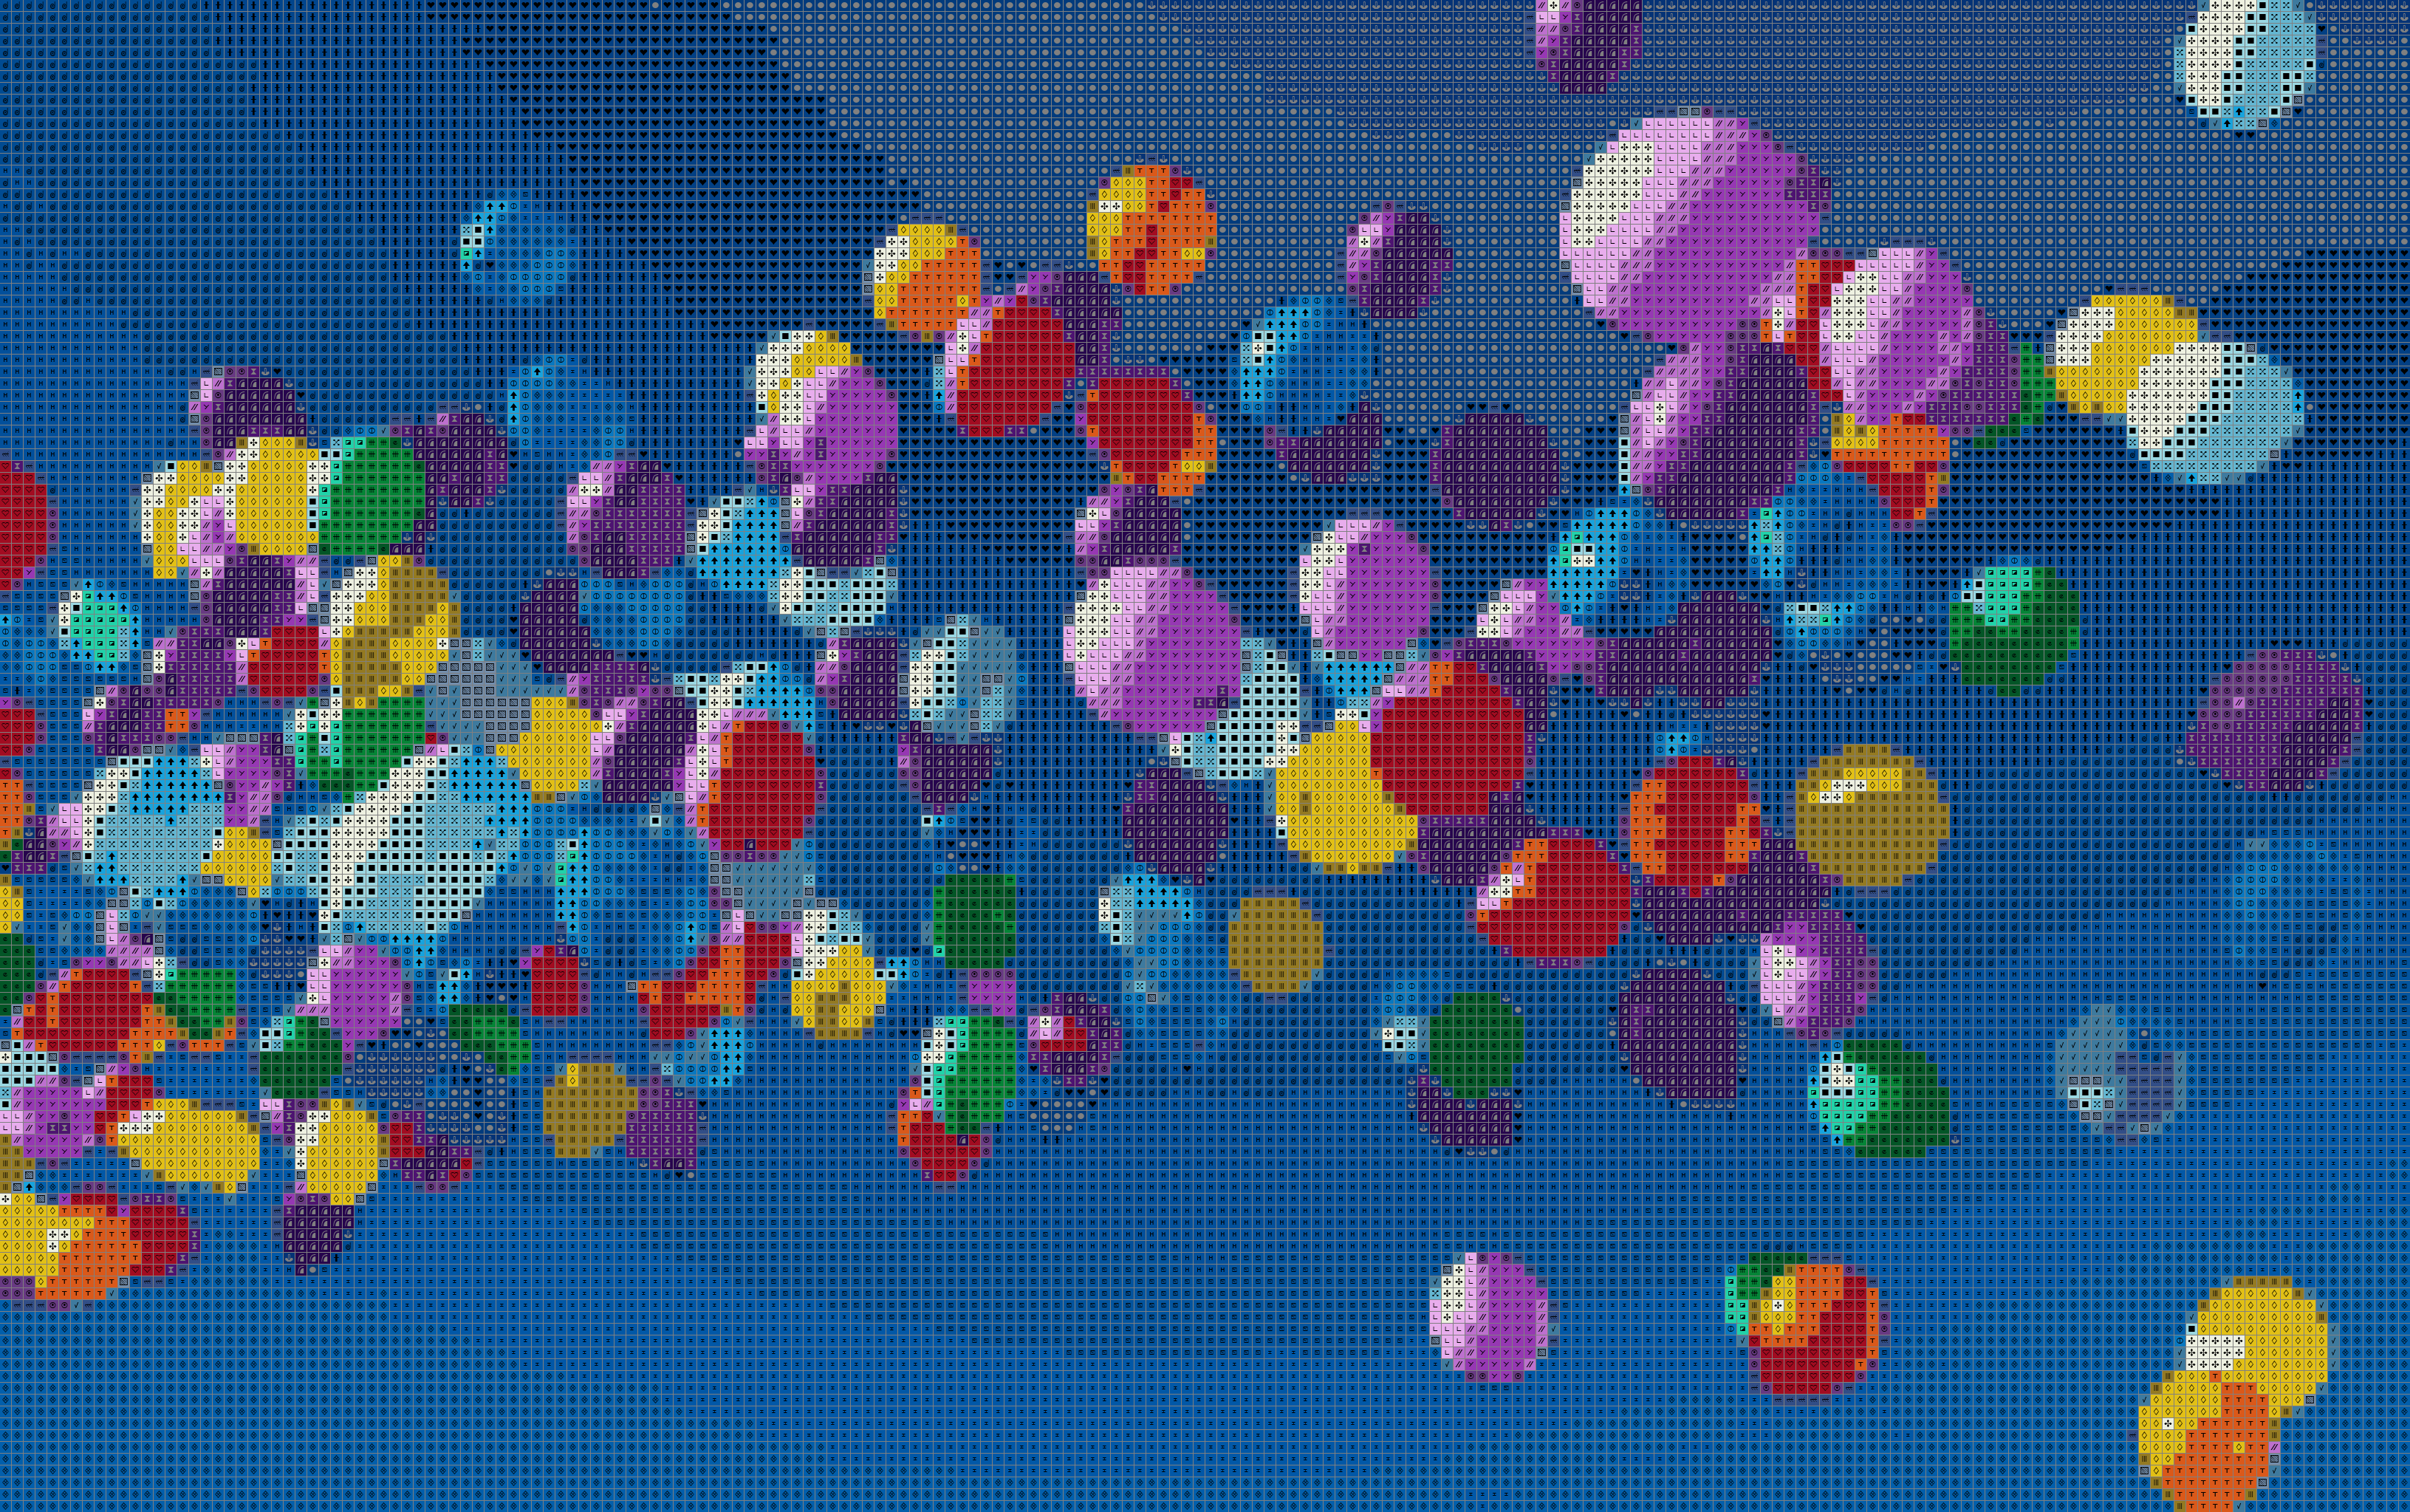
\includegraphics[width=130mm]{images/refactoring1/with_picto_baloons.png}
			\caption{Вариант схемы со значками для изображения baloons.png (30 цветов, 200 на 120)}
		}
	\end{figure}
	\label{with_picto_baloons}
	
	\begin{figure}[bh]
		\noindent\centering{
			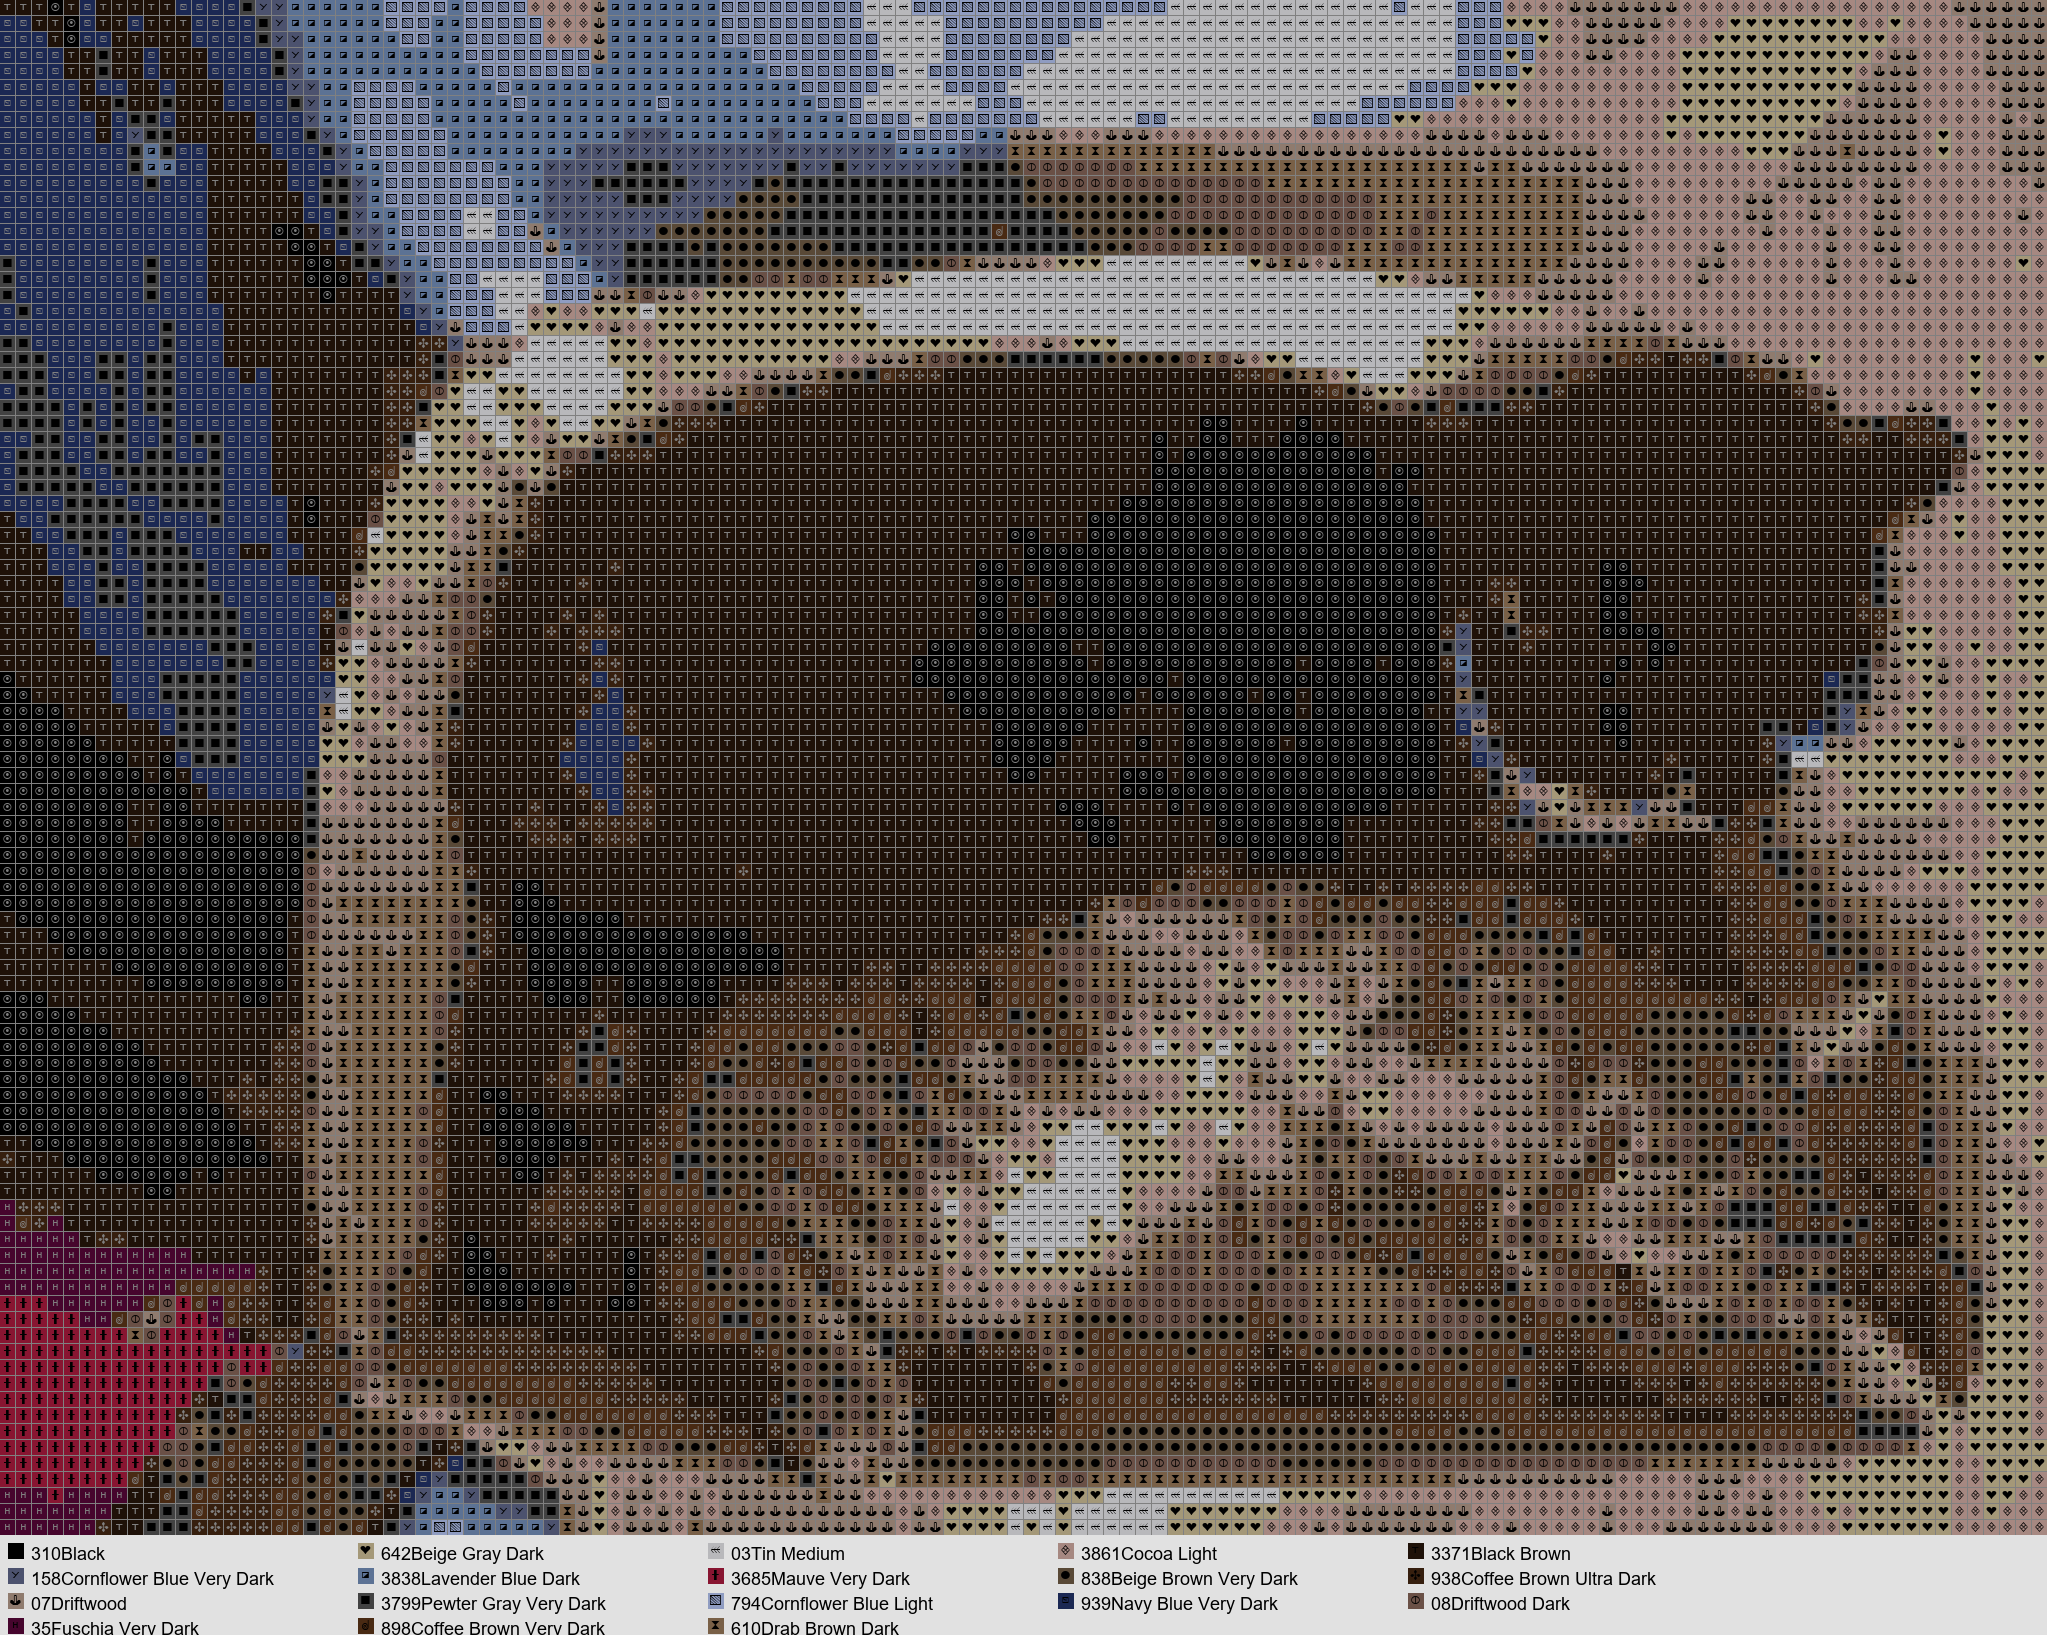
\includegraphics[width=130mm]{images/refactoring1/with_info_cats.png}
			\caption{Вариант схемы с информацией об используемых нитках для изображения cats.png}
		}
	\end{figure}
	\label{with_info_cats}
	
	\begin{figure}[bh]
		\noindent\centering{
			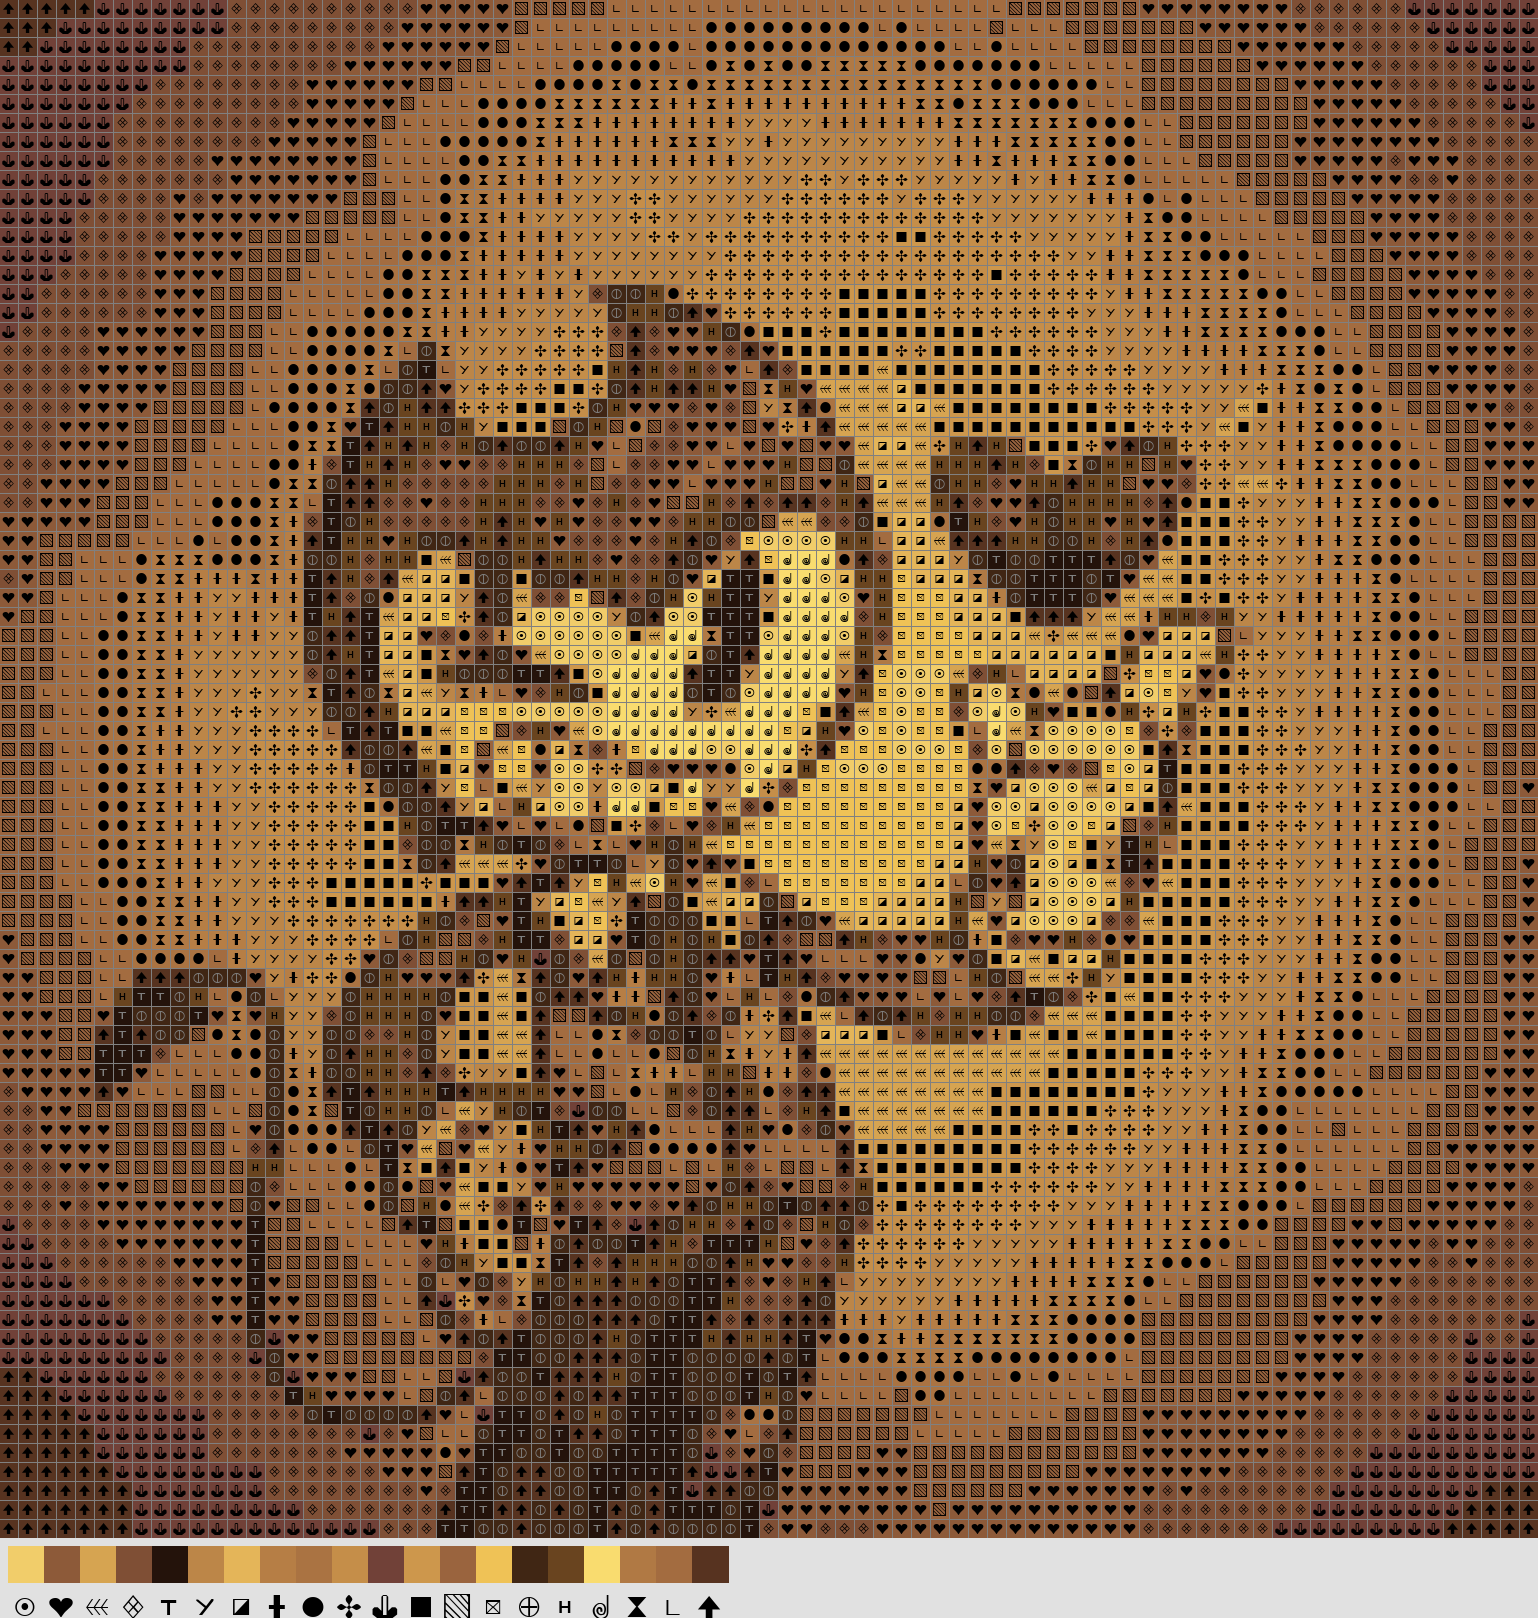
\includegraphics[width=130mm]{images/refactoring1/with_info_imp.png}
			\caption{Вариант схемы с информацией только о цветах для изображения imp.png}
		}
	\end{figure}
	\label{with_info_imp}
	
	\begin{figure}[bh]
		\noindent\centering{
			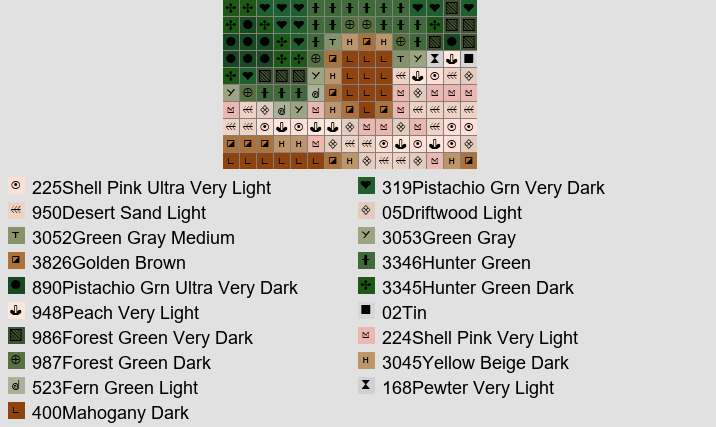
\includegraphics[width=130mm]{images/refactoring1/with_info_tiny.png}
			\caption{Вариант схемы с информацией об используемых нитках для очень маленького изображения}
		}
	\end{figure}
	\label{with_info_tiny}
	
\end{document}	